% !TEX root = main.tex
\documentclass[11pt,a4paper]{article}

\usepackage[margin=21mm]{geometry}
\usepackage[T1]{fontenc}
\usepackage{lmodern}
\usepackage{graphicx}
\usepackage{booktabs}
\usepackage{tabularx}
\usepackage{longtable}
\usepackage{array}
\usepackage{xcolor}
\usepackage{hyperref}
\usepackage{enumitem}
\usepackage{caption}
\usepackage{subcaption}
\usepackage{float}
\usepackage{fancyhdr}
\usepackage{amsmath}
\usepackage{pifont}

\definecolor{navy}{HTML}{183B56}
\definecolor{navydark}{HTML}{102838}
\definecolor{teal}{HTML}{168C8C}
\definecolor{orange}{HTML}{D17A22}
\definecolor{green}{HTML}{3F7D5A}
\definecolor{red}{HTML}{B84A4A}
\definecolor{lightblue}{HTML}{EDF4F7}
\definecolor{lightteal}{HTML}{EAF5F4}
\definecolor{lightorange}{HTML}{FFF2E4}
\definecolor{lightgreen}{HTML}{EDF6F0}
\definecolor{lightred}{HTML}{FCEEEE}
\definecolor{lightgray}{HTML}{F3F5F6}
\definecolor{darkgray}{HTML}{4C5661}

\hypersetup{
  colorlinks=true,
  linkcolor=navy,
  urlcolor=teal,
  citecolor=navy,
  pdfauthor={Felix Doublet},
  pdftitle={When Is It Too Late? A Scientific Experiment Plan for Causal VLA Recoverability},
  pdfsubject={SAFE, RoboCasa365, long-horizon failure detection, causal recoverability, and recovery guidance}
}

\captionsetup{font=small,labelfont=bf}
\setlist{leftmargin=1.45em,itemsep=0.25em,topsep=0.35em}
\setlength{\parskip}{0.48em}
\setlength{\parindent}{0pt}
\setlength{\headheight}{14pt}
\renewcommand{\arraystretch}{1.18}
\graphicspath{{figures/}}

\pagestyle{fancy}
\fancyhf{}
\lhead{Causal recoverability for long-horizon VLAs}
\rhead{Scientific experiment plan}
\cfoot{\thepage}

\newcolumntype{Y}{>{\raggedright\arraybackslash}X}
\newcolumntype{P}[1]{>{\raggedright\arraybackslash}p{#1}}
\newcommand{\code}[1]{\texttt{#1}}
\newcommand{\metric}[1]{\textbf{#1}}
\newcommand{\good}{\textcolor{green}{\ding{51}}}
\newcommand{\bad}{\textcolor{red}{\ding{55}}}
\newcommand{\planned}{\textcolor{orange}{\ding{108}}}

\newcommand{\boxednote}[4]{%
  \begin{center}
  \setlength{\fboxsep}{7pt}%
  \fcolorbox{#1}{#2}{%
    \begin{minipage}{0.91\textwidth}
    \textbf{#3}\quad #4
    \end{minipage}}
  \end{center}}

\newcommand{\sciencenote}[2]{\boxednote{teal}{lightteal}{#1}{#2}}
\newcommand{\implementationnote}[2]{\boxednote{navy}{lightblue}{#1}{#2}}
\newcommand{\positiveresult}[1]{\boxednote{green}{lightgreen}{Positive result.}{#1}}
\newcommand{\negativeresult}[1]{\boxednote{red}{lightred}{If the result is negative.}{#1}}
\newcommand{\cautionnote}[2]{\boxednote{orange}{lightorange}{#1}{#2}}

\newcommand{\phaseheader}[3]{%
  \clearpage
  \section{Phase #1: #2}
  \sciencenote{Scientific purpose.}{#3}}

\newcommand{\proposedfile}[1]{\path{#1}\textsuperscript{new}}

\begin{document}
\pagenumbering{roman}
\hypersetup{pageanchor=false}

\begin{titlepage}
\centering
\vspace*{16mm}
{\color{teal}\rule{\textwidth}{2.2pt}}\\[14mm]
{\Huge\bfseries\color{navydark} When Is It Too Late?\\[5mm]}
{\LARGE Causal Recoverability Curves for Long-Horizon\\Vision-Language-Action Manipulation}\\[14mm]
{\large\color{darkgray} A hypothesis-driven LaTeX experiment plan for adapting SAFE, measuring actionable warning time, learning recovery value, and evaluating critic-guided recovery on RoboCasa365}\\[17mm]
{\color{teal}\rule{\textwidth}{1.2pt}}\\[16mm]

\begin{tabular}{rl}
Primary target: & CoRL \\
Natural alternative: & ICRA \\
Stretch target: & RSS \\
Conditional vision route: & CVPR / ICCV / WACV \\
Primary policy: & Xiaomi-Robotics-1 on RoboCasa365 \\
Report date: & 26 August 2026 \\
\end{tabular}

\vfill
\begin{minipage}{0.9\textwidth}
\small
This document starts from the verified SAFE and recovery evidence already present in the repository. It incorporates the completed Phase~1 five-task frozen confirmation, the subsequent state-context development study, and the passing Phase~2 exact snapshot-replay validation. Phase~3 is now active as a bounded read-only candidate-opportunity analysis. The plan separates development evidence, retrospective analysis, frozen prospective shadow evaluation, simulator-oracle recovery, prospective intervention, and real-robot evidence. Every phase specifies the scientific hypothesis, the implementation required, the evaluation estimand, the statistical unit, the result that would count as positive, and the scientific meaning of a failed gate.
\end{minipage}
\vfill
{\small Felix Doublet --- Shinoda Laboratory}
\end{titlepage}
\hypersetup{pageanchor=true}

\tableofcontents
\clearpage
\pagenumbering{arabic}

\section{Executive recommendation}

\subsection{Recommended scientific thesis}

The research plan remains viable, but the central contribution should no longer be described as ``SAFE plus early triggering plus critic-guided flow.'' Recent work already studies calibrated VLA verification, recovery windows, counterfactual recovery labels, subtask backtracking, and critic- or reward-guided action generation~\cite{checkvla,b2ff,cyclevla,afil,rover,qvgm}. The stronger and more defensible thesis is:

\begin{quote}
\textbf{A failure detector's confidence is not its intervention value. Long-horizon VLA recovery has a state-, stage-, delay-, and operator-dependent deadline that must be measured causally and predicted directly.}
\end{quote}

The method should therefore learn whether intervention has positive value, when that value disappears, and which recovery action or operator should be selected. SAFE remains scientifically important as (i) the internal action-policy representation being adapted, (ii) a strong terminal-failure baseline, and (iii) a candidate input to the recovery-value model. It should not be assumed to be a value function.

\subsection{Primary paper endpoint}

The final primary endpoint is not detector ROC-AUC. It is the equal-task absolute improvement in final RoboCasa365 task success produced by the complete deployable system relative to the strongest frozen non-oracle baseline, under a matched intervention and inference budget. Detector ranking, warning time, stage recovery, and candidate-selection accuracy are mechanistic secondary endpoints that explain the task-success result.

\sciencenote{Recommended contribution statement.}{The paper introduces exact-prefix counterfactual recoverability curves, demonstrates that terminal-failure likelihood and causal intervention value diverge, and learns a stage-aware utility gate that decides whether, when, and how to recover while controlling harmful interventions.}

\subsection{Starting evidence}

Table~\ref{tab:starting-evidence} summarizes the evidence already available in the repository. The strongest current detector evidence is a frozen prospective Xiaomi shadow test, but it did not execute recovery. The five-task stage-aware development gain was tested on 250 new identity-disjoint parents and did not transfer. Phase~2 has since established exact complete-snapshot branching on a bounded two-task validation. The active dependency is therefore no longer replay engineering: it is whether the already-collected candidate branches contain enough causal outcome variation to justify a recovery critic.

\begin{table}[H]
\centering
\caption{Current evidence and the strongest defensible interpretation. ``Prospective shadow'' means the detector bundle was frozen before scoring new trajectories, but the detector did not change policy execution.}
\label{tab:starting-evidence}
\small
\begin{tabularx}{\textwidth}{P{0.22\textwidth}P{0.36\textwidth}Y}
\toprule
Component & Evidence & Current interpretation \\
\midrule
Xiaomi matched-FPR shadow test & 760 balanced primary rollouts. Staged SAFE plus time reached TPR 0.668 at FPR 0.050, versus time-only TPR 0.632 at FPR 0.047. The timing gain was 0.0259 task horizons and its bootstrap interval crossed zero; only 2.9\% of failures were detected by the 25\% landmark. & Modest prospective classification gain; overall early-warning gate failed; no recovery claim. \\
Full-parent stage-aware confirmation & Development selection favored conditioned SAFE (ROC 0.696 versus 0.592 terminal). On 250 frozen, identity-disjoint parents, conditioned SAFE reached 0.489 versus 0.523 terminal, 0.563 SAFE38, and 0.500 time-only. All preregistered gates failed. & The development gain did not replicate. Predicate-stage-aware SAFE remains a baseline or model input, not a deployable trigger contribution. \\
State-context follow-up & A new 250-parent cohort recorded a 240-dimensional proprioceptive state history. Development selected stage SAFE at 0.693, context at 0.691, and terminal at 0.690. On the locked 85-parent retrospective holdout, stage reached 0.584, context 0.566, terminal 0.470, and time-only 0.500; both primary contrast intervals crossed zero. & Descriptive evidence of task-specific signal, not prospective confirmation. State context did not improve the selected ranking or the matched-FPR operating point. \\
RLDX Subtask-SAFE & Raw segment ROC 0.734 fell to parent-aware ROC 0.558, while an elapsed-time baseline reached 0.740. Frozen causal-prefix variants remained near chance. & Retrospective segment separation did not translate to online intervention evidence. \\
Recovery infrastructure & Ordered subtask anchors, environment reset, EEF recovery, continuation, and Xiaomi deterministic best-of-$K$ proposals exist. & Useful implementation base; existing runs do not establish randomized recovery utility. \\
Complete snapshot replay & On two tasks, 10 of 10 eligible parents produced 20 of 20 snapshots and 140 of 140 branches: 80 explicit candidates, 40 same-seed repeats, and 20 environment-only controls. There were zero branch errors, exact repeated requests/actions/observations/causal transitions, 100\% repeated-suffix agreement, and 100\% candidate diversity. & Phase~2 engineering validity passed. The branches are causally aligned simulator evidence, but candidate recovery utility has not yet been measured. \\
\bottomrule
\end{tabularx}
\end{table}

\begin{figure}[H]
\centering
\begin{subfigure}[t]{0.48\textwidth}
  \centering
  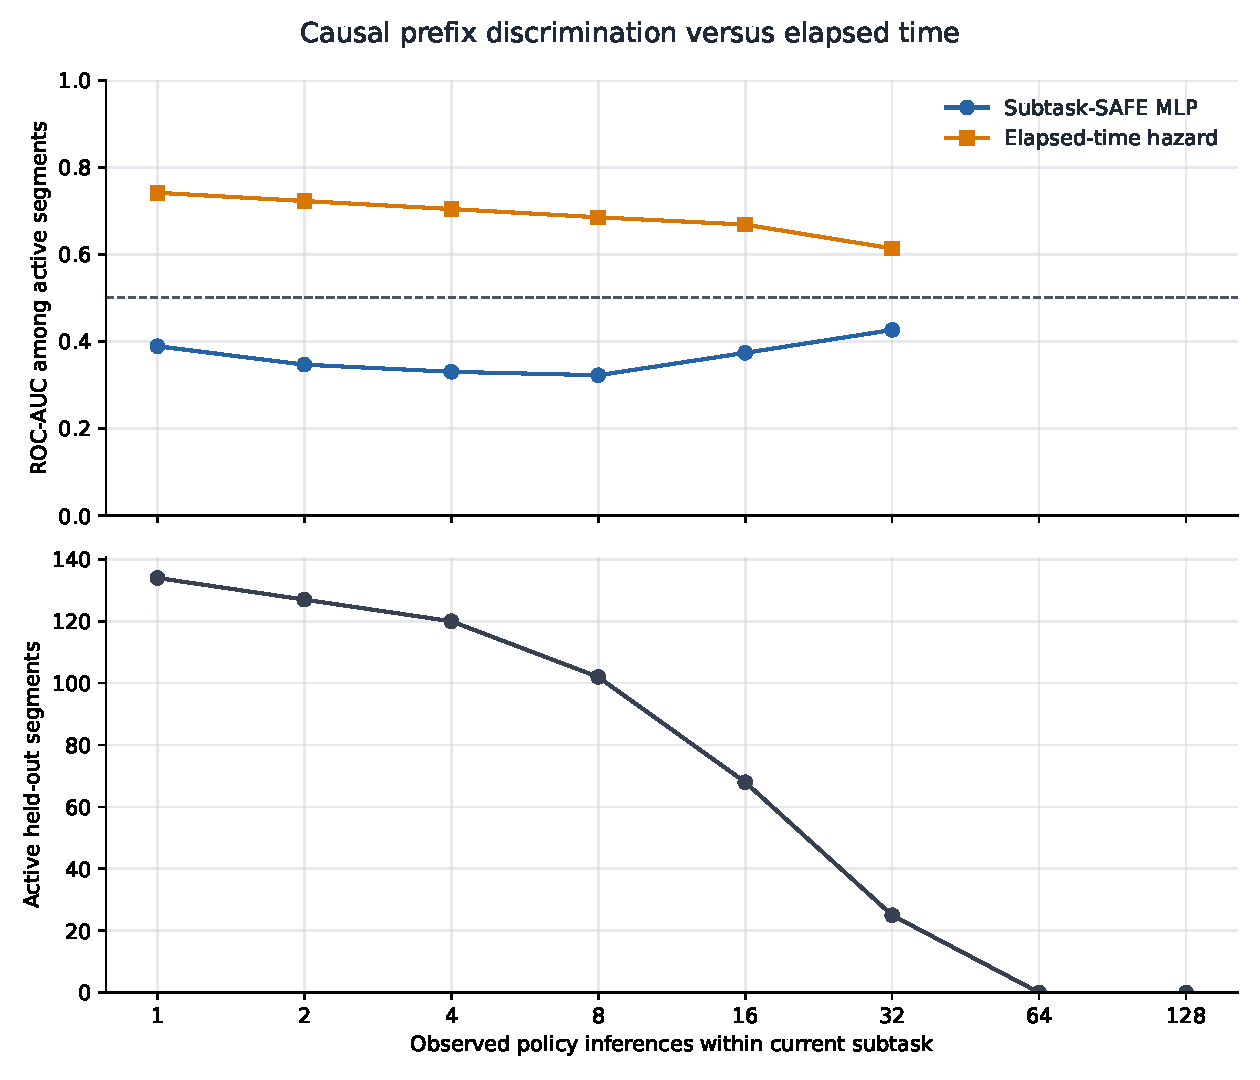
\includegraphics[width=\linewidth]{subtask_causal_prefix_roc.pdf}
  \caption{Causal prefix evaluation exposes the gap between retrospective Subtask-SAFE ranking and online utility.}
\end{subfigure}\hfill
\begin{subfigure}[t]{0.48\textwidth}
  \centering
  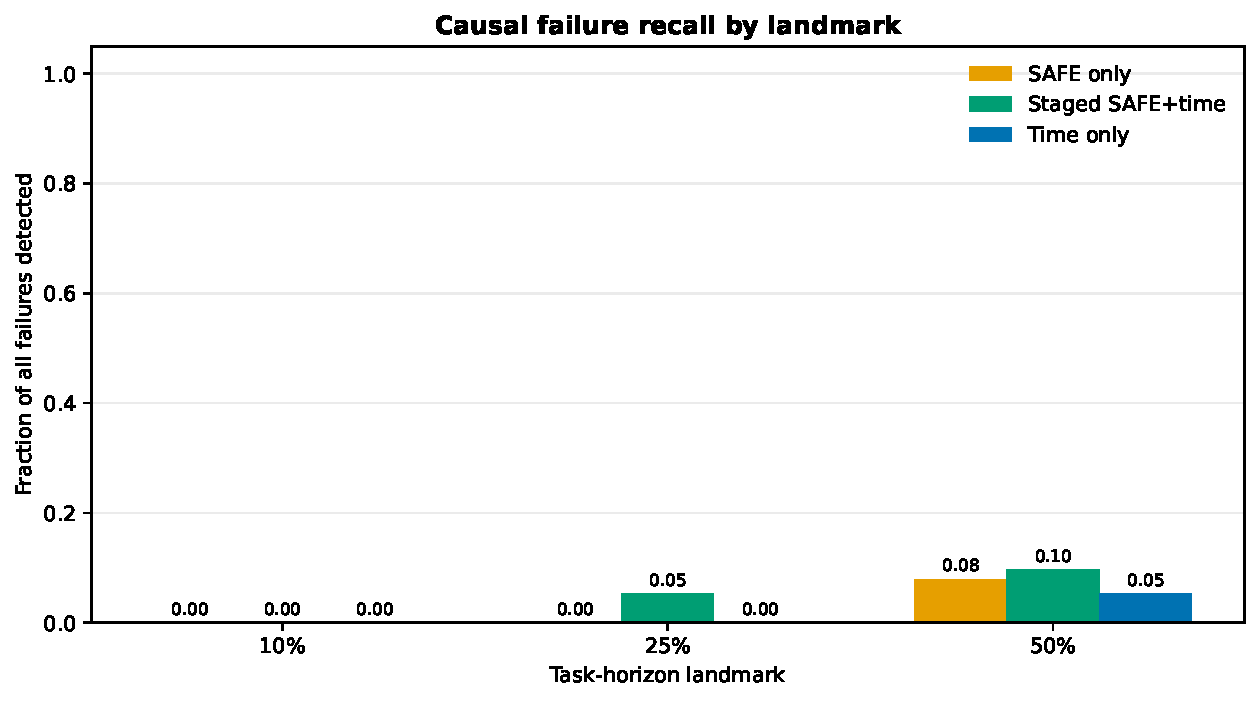
\includegraphics[width=\linewidth]{xr1_matched_fpr_recall_by_landmark.pdf}
  \caption{The frozen Xiaomi shadow test achieved low early-landmark recall on composite failures.}
\end{subfigure}
\caption{The research plan begins from negative causal and timing evidence rather than from retrospective ROC alone. Figures are reproduced from the checksum-backed full report.}
\label{fig:starting-point}
\end{figure}

\subsection{Dependency-gated roadmap}

\begin{longtable}{P{0.07\textwidth}P{0.28\textwidth}P{0.28\textwidth}P{0.269\textwidth}}
\caption{Experiment dependency structure. Each expensive phase is conditional on the preceding scientific or engineering gate.}\label{tab:roadmap}\\
\toprule
Phase & Experiment & Positive result & If the gate fails \\
\midrule
\endfirsthead
\toprule
Phase & Experiment & Positive result & If the gate fails \\
\midrule
\endhead
0 & Protocol freeze and evidence audit & Artifacts, identities, and endpoints are immutable and reproducible. & Repair integrity; do not collect. \\
1 & Frozen stage-aware confirmation \bad & Early stage-aware ranking transfers to new parents. & \textbf{Observed: gate failed.} SAFE becomes a baseline/input, not the trigger contribution. \\
2 & Complete snapshot replay \good & \textbf{Observed: gate passed.} Same state and randomness reproduced while declared candidate seeds created controlled alternatives. & Not applicable; preserve the passing bundle and hashes. \\
3 & Counterfactual opportunity screen \planned & Candidate choice changes recovery outcome with substantial oracle headroom. & Change proposal distribution, timing, or recovery operator before critic training. \\
4 & Recoverability surfaces & Intervention value varies meaningfully with delay, stage, and operator. & Narrow to a diagnostic benchmark or improve operators. \\
5 & Recovery-value critic & The learned critic predicts and ranks causal utility on sealed parents/tasks. & Do not guide the policy; preserve the benchmark result. \\
6 & Prospective best-of-$K$ selection & Critic selection beats random $K=4$ under identical candidates. & No flow guidance; critic is not actionably causal. \\
7 & Frozen end-to-end intervention & Final task success improves without excessive harm. & No deployable recovery-system claim. \\
8 & Differentiable flow guidance & Guided $K=1$ matches critic $K=4$ at lower cost and no safety loss. & Retain discrete critic reranking. \\
9 & Generalization and physical validation & Benefit survives held-out tasks/scenes and another policy or robot. & Scope the paper to same-policy RoboCasa365. \\
\bottomrule
\end{longtable}

\cautionnote{Planning thresholds.}{The numerical gates in this report are proposed research decisions, not official venue requirements. Final powered sample sizes must be frozen from blinded pilot variance and the exact hierarchical analysis.}

\sciencenote{Current decision.}{Freeze the passing Phase~2 run and start Phase~3 with a read-only analysis of its 20 paired snapshots and 80 explicit candidate branches. This two-task pilot can estimate mixed-outcome frequency and oracle headroom, but cannot satisfy the formal requirement for mixed outcomes in at least three of five tasks. Scale to the predeclared five-task opportunity study only if the bounded pilot reaches at least 20\% mixed snapshots and at least 15 percentage points of oracle-over-random headroom. Do not train a critic before that gate.}

\section{Formal scientific framework}

\subsection{Failure risk and recovery value are different estimands}

Let $h_t$ denote all causal information available at genuine policy inference $t$: observations, proprioception, task language, executed action history, current cached-plan state, and any online stage estimate. Let $Y\in\{0,1\}$ denote eventual full-task success. A conventional failure monitor estimates
\begin{equation}
  p_{\mathrm{fail}}(h_t) = \Pr(Y=0\mid h_t).
\end{equation}
This quantity can be high even when no available recovery action improves outcome, and it can be low while a cheap early intervention would be beneficial. The proposed causal object is intervention-specific recoverability. For recovery operator $k$ applied after delay $d$,
\begin{equation}
  R_k(h_t,d) = \Pr\!(Y=1\mid \operatorname{do}(k\text{ at }t+d),h_t).
  \label{eq:recoverability}
\end{equation}
The intervention advantage is
\begin{equation}
  \Delta_k(h_t,d)
  = R_k(h_t,d)-R_{\mathrm{continue}}(h_t,d)
  -\lambda C_k-\mu H_k,
  \label{eq:advantage}
\end{equation}
where $C_k$ is compute or latency cost, $H_k$ is intervention harm, and $\lambda,\mu$ are frozen decision weights. A deployable controller intervenes only when the lower-confidence estimate of $\max_k\Delta_k$ exceeds a predeclared threshold, and chooses the operator with the largest predicted value.

\subsection{Recovery deadline}

The project should not assume that recoverability decays monotonically. A policy may self-correct, enter a more controllable state, or transition between stages. For a positive-value margin $\epsilon$, define the sampled operational deadline
\begin{equation}
  D_k(h_t;\epsilon)
  = \sup\{d\in\mathcal{D}:\Delta_k(h_t,d)>\epsilon\},
  \label{eq:deadline}
\end{equation}
where $\mathcal{D}$ is a prespecified delay grid in genuine policy inferences. The scientific question is therefore not simply whether ``earlier is better,'' but how $D_k$ and the shape of $\Delta_k(h_t,d)$ depend on task, stage, failure mode, and operator.

\subsection{Counterfactual identification in simulation}

For snapshot $i$, candidate/operator $k$, delay $d$, and common-randomness schedule $\omega$, let $Y_i(k,d;\omega)$ be the potential suffix outcome. RoboCasa simulation permits repeated branches from an identical state. This does not identify every real-world causal effect, but it permits controlled estimation of within-simulator intervention contrasts when four conditions hold:
\begin{enumerate}
  \item the simulator and policy state are fully restored;
  \item intervention branches share the same environment and fallback-policy randomness until treatment induces divergence;
  \item branch states are selected independently of the detector being evaluated;
  \item all branches, including homogeneous candidate sets and harmful interventions, are retained.
\end{enumerate}
Under these conditions, the paired branch contrast
\begin{equation}
  Y_i(k,d;\omega)-Y_i(\mathrm{continue},d;\omega)
\end{equation}
is the fundamental training and evaluation signal. The top-level population claim still requires resampling tasks and parents; thousands of candidate branches do not create thousands of independent tasks.

\subsection{Experimental hierarchy}

\begin{table}[H]
\centering
\caption{Statistical hierarchy and grouping rules.}
\label{tab:hierarchy}
\small
\begin{tabularx}{\textwidth}{P{0.20\textwidth}P{0.34\textwidth}Y}
\toprule
Unit & Definition & Required rule \\
\midrule
Task & One RoboCasa365 task identity and its semantic-stage catalog. & Top-level resampling unit for cross-task claims. \\
Parent & One original rollout identified by task, environment seed, reset index, and policy-sampling family. & Split before extracting stages, prefixes, or snapshots. \\
Snapshot & One complete causal simulator-policy state nested within a parent. & Every operator and candidate branch stays in the same split. \\
Candidate branch & One action chunk or recovery operator executed after restoration. & Paired observation, not an independent sample. \\
Inference & One genuine policy model request. & Store one SAFE/context feature; cached actions do not create new samples. \\
Model seed & One neural initialization. & Measures training instability, not environment or task replication. \\
\bottomrule
\end{tabularx}
\end{table}

\subsection{Primary estimands}

\paragraph{Frozen detector confirmation.}
At exact active-stage prefixes 1 and 2, define the task-and-stage macro ROC $\theta_{\mathrm{rank}}$, with equal weight for every supported task-stage stratum. The primary contrast is
\begin{equation}
  \Delta_{\mathrm{rank}}
  = \theta_{\mathrm{conditioned}}-\theta_{\mathrm{terminal}}.
\end{equation}

\paragraph{Candidate actionability.}
For identical candidate sets,
\begin{equation}
  \Delta_K
  = \Pr(Y=1\mid K=4,\text{critic})
  -\Pr(Y=1\mid K=4,\text{random}).
\end{equation}

\paragraph{End-to-end task success.}
For method $a$ and frozen control $c$, the primary deployment estimand is the equal-task treatment effect
\begin{equation}
  \Delta_{\mathrm{success}}
  = \operatorname{mean}_{i\in\mathcal{T}}
  [\Pr(Y=1\mid A=a,i)-\Pr(Y=1\mid A=c,i)].
  \label{eq:task-effect}
\end{equation}

\paragraph{Successful-parent harm.}
The safety quantity is episode-level: a would-be successful parent that is made unsuccessful by intervention counts as harm. Per-inference false-positive rate is secondary and cannot replace this unit.

\subsection{Evidence labels}

Every result table and caption should label evidence as one of: \emph{development selection}, \emph{retrospective locked}, \emph{prospective shadow}, \emph{prospective randomized intervention}, \emph{simulator oracle}, or \emph{physical deployment}. Local unit tests and source inspection establish implementation properties only; they are not simulator or policy-performance evidence.

\phaseheader{0}{Freeze the protocol and audit experimental readiness}{Establish an immutable, machine-auditable foundation before any new scientific outcome is observed. This phase prevents hidden model selection, identity reuse, path drift, and accidental promotion of a development result into a confirmation claim.}

\subsection{Scientific rationale}

Phase 0 has no performance hypothesis. Its role is to make every later hypothesis falsifiable. A confirmatory result is interpretable only when the policy, feature layer, model, score transformation, task/stage catalog, prefixes, thresholds, seed families, retry rules, and statistical code were fixed before outcomes. Integrity failures are engineering failures, not negative scientific findings.

The current project spans local source code, cluster source, durable artifacts, multiple policy families, and several already opened cohorts. Therefore, the protocol must explicitly distinguish the 170-parent stage-aware development allocation, the opened 80-parent outer set, the prospective Xiaomi shadow cohort, new confirmation identities, critic development identities, calibration identities, and final randomized-intervention identities.

\subsection{What must be implemented}

\begin{enumerate}
  \item \textbf{Protocol manifest.} Add a machine-readable manifest containing repository commits, policy/checkpoint hashes, SAFE revision, task and stage catalogs, feature layer and aggregation, prefixes, model seeds, normalization, thresholds, candidate count, replan length, recovery horizon, primary endpoint, primary comparison, and bootstrap seed.
  \item \textbf{Identity registry.} Represent each parent by the tuple
  \[
    (\text{task},\text{environment seed},\text{reset index},\text{policy-sampling family}).
  \]
  The registry must reject overlap across development, selection, calibration, confirmation, critic test, and final intervention roles.
  \item \textbf{Artifact validation.} Verify checksums for the Xiaomi checkpoint, SAFE checkpoints, runtime bundles, server patches, and source commits. Refuse to run if a frozen artifact differs.
  \item \textbf{Action-equivalence smoke.} Confirm that requesting SAFE/context features with an identical sampling seed does not change the decoded action chunk relative to the action-only request.
  \item \textbf{Run metadata.} Every run must store exact command, task list, code revision, checkpoint, seed/reset allocation, GPU and port mapping, model-loaded log, output path, and partial/error status.
\end{enumerate}

\implementationnote{Existing modules to reuse.}{Use \path{docs/cluster_experiment_runbook.md}, \path{robocasa/recovery/safe/run_stage_aware_parent_safe.py}, \path{robocasa/recovery/safe/stage_aware_parent_safe.py}, \path{robocasa/recovery/xiaomi_robotics_1_policy.py}, and the current dataset/schema validators.}

\implementationnote{Proposed additions.}{Add \proposedfile{robocasa/recovery/safe/experiment_protocol.py} for schema validation and \proposedfile{robocasa/recovery/safe/audit_experiment_identities.py} for cross-manifest overlap checks. Add unit tests that deliberately alter a checksum, reuse a seed/reset identity, change a frozen prefix, and duplicate one inference record.}

\subsection{Evaluation}

Phase 0 is evaluated with deterministic integrity tests rather than ROC or success rate. The required checks are listed in Table~\ref{tab:phase0-checks}.

\begin{table}[H]
\centering
\caption{Phase 0 readiness checks.}
\label{tab:phase0-checks}
\small
\begin{tabularx}{\textwidth}{P{0.28\textwidth}Y P{0.20\textwidth}}
\toprule
Check & Evaluation & Positive criterion \\
\midrule
Artifact integrity & Recompute hashes and reload every frozen runtime. & Exact hash agreement; strict model loading. \\
Identity disjointness & Compare all role manifests by rollout ID and task/seed/reset tuple. & Zero overlap. \\
Feature/action alignment & Repeat seeded action-only and feature-return requests. & Numerically identical decoded action. \\
Inference sampling & Count genuine server requests and stored feature records. & Exactly one feature per genuine inference. \\
Cluster preflight & Verify storage, model-loaded log, listening port, server/GPU process, and one bounded rollout. & Zero traceback; complete output and manifest. \\
Analysis determinism & Re-run the frozen scorer and bootstrap with the same seed. & Identical scores and intervals within numerical tolerance. \\
\bottomrule
\end{tabularx}
\end{table}

\positiveresult{All frozen artifacts resolve, identity roles are disjoint, the feature-return path is action-equivalent, and one bounded live rollout produces aligned policy, feature, stage, and outcome records. This result establishes experimental readiness only; it does not support a detector or recovery claim.}

\negativeresult{Stop new collection. Repair provenance, state alignment, server compatibility, storage, or identity allocation without changing the scientific endpoints. A Phase 0 failure invalidates the affected experiment rather than falsifying a scientific hypothesis.}

\subsection{Required artifacts}

\begin{itemize}
  \item \path{protocol.json} and a human-readable protocol summary;
  \item \path{allocation_manifest.jsonl} with all planned arms and identities;
  \item \path{artifact_checksums.json} and source/checkpoint revisions;
  \item preflight and one-rollout smoke logs under durable \path{/gs/bs} storage;
  \item a PASS/FAIL audit report generated before Phase 1 outcomes are opened.
\end{itemize}

\phaseheader{1}{Frozen confirmation of full-parent predicate-stage-aware SAFE}{\textbf{Completed; confirmatory gate failed.} The promising 0.696 development result was tested on 250 genuinely new parent and seed/reset identities without refitting, renormalization, threshold update, or stage-support change. The result did not transfer.}

\subsection{Scientific hypothesis}

The working explanation for composite-task difficulty is label and temporal-context misalignment. Terminal labels ask whether the entire parent eventually fails. Subtask-SAFE evaluated on independent stage windows discards the parent history and broadcasts an eventual stage outcome across all early samples. The proposed correction preserves the full parent trajectory while conditioning the representation on active stage, stage-anchor feature change, causal progress, task/stage identity, and near-failure horizons. In the current evaluator, however, active-stage labels come from simulator predicates. They therefore provide an oracle-stage estimate of representation quality and must not be confused with a causal online stage estimate.

The confirmatory hypothesis is
\begin{equation}
  H_1:\quad
  \Delta_{\mathrm{rank}}
  = \theta_{\mathrm{conditioned}}
  -\theta_{\mathrm{terminal}}>0,
\end{equation}
where $\theta$ is the equal-task/equal-stage ROC averaged over exact active-stage prefixes 1 and 2. A positive result would demonstrate early stage-specific ranking signal. It would not yet demonstrate calibrated online warning or recovery utility.

\subsection{Completed implementation and frozen protocol}

The confirmation path collected a pristine context-enabled cohort and enforced the frozen runtime contract.

\begin{enumerate}
  \item Fifty fixed-attempt parents were retained for each of the five predeclared composite tasks: 250 parents total, 120 successes and 130 failures. The task names and effects are reported in Table~\ref{tab:phase1-context-by-task}.
  \item The seed/reset family was disjoint from the 170 development parents and the opened 80-parent outer set. Every valid attempt was retained.
  \item Raw Xiaomi SAFE features, decoded action chunks, semantic traces, and causal state history were recorded. The context is a 240-dimensional flattened proprioceptive state history, not RGB or a visual embedding, and it was forbidden as an input to the frozen confirmation.
  \item The frozen conditioned, terminal, multihorizon, stage, prototype, time-only, and broad SAFE38 comparators were applied. No model, normalizer, threshold, supported-stage rule, or score transformation was updated on test.
  \item The evaluation contained 431 stage events. One failed parent ended in a failed stage with zero genuine policy inferences; it was reported as causally unobserved rather than imputed or silently dropped.
\end{enumerate}

\implementationnote{Existing implementation.}{The primary entry point is \path{robocasa/recovery/safe/run_stage_aware_parent_safe.py} in \code{evaluate} mode, with modeling and grouped metrics in \path{robocasa/recovery/safe/stage_aware_parent_safe.py}. The frozen procedure is documented in \path{docs/safe_xiaomi_stage_aware_parent.md}.}

\implementationnote{Tests to add or retain.}{Tests must verify exact rollout-ID agreement for external SAFE38 scores, rejection of development identity reuse, prohibition of test-time threshold updates, exact prefix aggregation, task/stage macro weighting, and preservation of the context channel without reading it in the confirmation arm.}

\cautionnote{Deployability boundary.}{A positive result in this phase authorizes a simulator-predicate-stage-conditioned upper bound only. Phase 5 must replace predicate stage with a frozen causal stage tracker and quantify the oracle-versus-predicted-stage gap before the method can be used online.}

\subsection{Frozen confirmation result}

\begin{table}[H]
\centering
\caption{Development selection versus frozen identity-disjoint confirmation. ROC-AUC is the equal-task/equal-stage average over active-stage prefixes 1 and 2. Confidence intervals are hierarchical task/parent bootstrap intervals for the paired contrast.}
\label{tab:phase1-confirmation}
\small
\begin{tabularx}{\textwidth}{P{0.24\textwidth}P{0.19\textwidth}P{0.21\textwidth}Y}
\toprule
Quantity & Development & Frozen confirmation & Interpretation \\
\midrule
Parents & 170 total; 37 selection & 250 identity-disjoint & Confirmation identities were never used for fitting or selection. \\
Conditioned SAFE ROC & 0.696 & 0.489 & The development advantage did not transfer. \\
Terminal SAFE ROC & 0.592 & 0.523 & Terminal SAFE exceeded conditioned SAFE on confirmation. \\
SAFE38 independent ROC & Not primary & 0.563 & Best frozen SAFE comparator, but still only modest early ranking. \\
Time-only ROC & 0.500 & 0.500 & Exact early prefixes remove elapsed-time ranking by construction. \\
Conditioned minus terminal & $+0.104$ descriptive & $-0.034$; 95\% CI $[-0.146,+0.076]$ & Direction reversed and interval crossed zero. \\
Conditioned minus time & $+0.196$ descriptive & $-0.011$; 95\% CI $[-0.119,+0.112]$ & No evidence beyond the time control. \\
Conditioned minus SAFE38 & Not frozen & $-0.073$; 95\% CI $[-0.243,+0.111]$ & No advantage over the broad frozen detector. \\
\bottomrule
\end{tabularx}
\end{table}

At the frozen matched-FPR operating point, conditioned SAFE reached failed-stage TPR 0.145 at successful-parent FPR 0.067, compared with time-only TPR 0.504 at FPR 0.033. Miss-adjusted detection fraction was 0.965 for conditioned SAFE and 1.000 for time-only, where a lower fraction is earlier. Thus the detector was neither more sensitive nor operationally earlier than the time baseline.

\begin{table}[H]
\centering
\caption{Preregistered Phase~1 gate audit. Every criterion was evaluated without test-time updates.}
\label{tab:phase1-gates}
\small
\begin{tabularx}{\textwidth}{Y P{0.25\textwidth}P{0.12\textwidth}}
\toprule
Criterion & Observed & Verdict \\
\midrule
Conditioned macro ROC at least 0.60 & 0.489 & \bad \\
Conditioned minus terminal at least $+0.05$ & $-0.034$ & \bad \\
Hierarchical 95\% interval entirely above zero & $[-0.146,+0.076]$ & \bad \\
Conditioned beats terminal on at least four of five tasks & 2 of 5 & \bad \\
Conditioned beats time-only on at least four of five tasks & 2 of 5 & \bad \\
Matched-FPR TPR no more than 0.05 below time & difference $-0.359$ & \bad \\
\bottomrule
\end{tabularx}
\end{table}

\negativeresult{The preregistered Phase~1 result is negative. Treat the 0.696 development ROC as selection noise or cohort-specific structure. Do not refit on the confirmation parents, promote conditioned SAFE as a deployable trigger, or start another broad detector sweep on this cohort. SAFE remains a baseline and a possible input to a later recovery-value model.}

\subsection{Post-confirmation state-context development study}

After the frozen failure was published, the 250-parent context-enabled cohort was used for a new, explicitly developmental study. It was repartitioned into 92 fit, 35 selection, 38 calibration, and 85 locked retrospective-holdout parents. Because this study began after the cohort had already been scored in the frozen confirmation, the 85-parent result is \emph{retrospective locked-holdout evidence}, not a new prospective claim.

Sixty screening fits and 15 refits compared terminal, stage, multihorizon, conditioned, and state-context arms. The selection ROC values were 0.690 terminal, 0.693 stage, 0.685 multihorizon, 0.653 conditioned, and 0.691 context. Stage was selected, but its advantage over context was only 0.002 and over terminal only 0.003, both smaller than the observed seed variation.

On the frozen 85-parent holdout, stage reached prefix-1/2 macro ROC 0.584, context 0.566, terminal 0.470, and time-only 0.500. Stage minus terminal was $+0.113$ with 95\% CI $[-0.075,+0.300]$; stage minus time was $+0.084$ with 95\% CI $[-0.118,+0.267]$. Stage beat terminal on four tasks but time on only three, and its macro ROC remained below the predeclared 0.60 gate. At matched FPR, stage had failed-stage TPR 0.100 at parent FPR 0.049, versus time-only TPR 0.125 at FPR 0.024. Its miss-adjusted timing contrast versus time was $-0.014$ with 95\% CI $[-0.064,0.000]$. All preregistered operational criteria failed.

\begin{table}[H]
\centering
\caption{Retrospective 85-parent prefix-1/2 ROC-AUC by task. These heterogeneous effects are descriptive and not multiplicity-adjusted.}
\label{tab:phase1-context-by-task}
\small
\begin{tabular}{lrrrrrr}
\toprule
Task & Stage & Context & Conditioned & Multi & Terminal & Time \\
\midrule
ArrangeBreadBasket & 0.316 & 0.173 & 0.279 & 0.368 & 0.376 & 0.500 \\
ArrangeTea & 0.625 & 0.712 & 0.673 & 0.567 & 0.404 & 0.500 \\
BreadSelection & 0.482 & 0.569 & 0.565 & 0.431 & 0.324 & 0.500 \\
CuttingToolSelection & 0.838 & 0.709 & 0.675 & 0.849 & 0.613 & 0.500 \\
GarnishPancake & 0.657 & 0.664 & 0.743 & 0.686 & 0.636 & 0.500 \\
\bottomrule
\end{tabular}
\end{table}

\begin{table}[H]
\centering
\caption{Retrospective prefix-1/2 ROC-AUC by supported semantic stage. Support is the number of evaluable stage events in the 85-parent holdout; sparse rows are descriptive only.}
\label{tab:phase1-context-by-stage}
\scriptsize
\begin{tabularx}{\textwidth}{Y rrrrr}
\toprule
Task and semantic stage & Support & Stage & Context & Terminal & Time \\
\midrule
ArrangeBreadBasket: OpenCabinet\_1 & 16 & 0.250 & 0.089 & 0.643 & 0.500 \\
ArrangeBreadBasket: PickPlaceCabinetToCounter\_2\_place & 7 & 0.333 & 0.083 & 0.042 & 0.500 \\
ArrangeBreadBasket: PickPlaceCounterToCounter\_3\_place & 15 & 0.365 & 0.346 & 0.442 & 0.500 \\
ArrangeTea: PickPlaceCabinetToCounter\_2\_place & 17 & 0.625 & 0.712 & 0.404 & 0.500 \\
BreadSelection: PickPlaceCabinetToCounter\_2\_place & 14 & 0.488 & 0.450 & 0.363 & 0.500 \\
BreadSelection: PickPlaceCabinetToCounter\_2\_release & 5 & 0.625 & 0.875 & 0.125 & 0.500 \\
BreadSelection: PickPlaceCounterToCounter\_1\_place & 17 & 0.333 & 0.383 & 0.483 & 0.500 \\
CuttingToolSelection: OpenDrawer\_1 & 17 & 0.697 & 0.689 & 0.538 & 0.500 \\
CuttingToolSelection: PickPlaceDrawerToCounter\_2\_place & 11 & 0.979 & 0.729 & 0.688 & 0.500 \\
GarnishPancake: strawberry\_on\_pancake & 17 & 0.657 & 0.664 & 0.636 & 0.500 \\
\bottomrule
\end{tabularx}
\end{table}

The task audit identifies a real scientific diagnostic rather than a general detector win. Stage-aware scoring was strong for \code{CuttingToolSelection} and positive for \code{ArrangeTea} and \code{GarnishPancake}, but failed sharply for \code{ArrangeBreadBasket}. Within \code{ArrangeBreadBasket}, stage ROC ranged from 0.250 for \code{OpenCabinet\_1} to 0.365 for the third placement stage; state context fell to 0.089 on \code{OpenCabinet\_1}. Conversely, \code{CuttingToolSelection::PickPlaceDrawerToCounter\_2\_place} reached stage ROC 0.979. A sparse five-event BreadSelection release stage produced context ROC 0.875 and must not be treated as stable evidence. This heterogeneity argues for measuring intervention value by state and operator, not for adding more global stage-label complexity.

\cautionnote{Interpretation of state context.}{The recorded context is proprioceptive state history only. It did not beat the selected stage arm on the locked holdout and does not establish a visual-context contribution. Any future visual ablation requires causal RGB embeddings and a new untouched cohort.}

\subsection{Evaluation design}

\begin{table}[H]
\centering
\caption{Frozen stage-aware confirmation design.}
\label{tab:phase1-design}
\small
\begin{tabularx}{\textwidth}{P{0.26\textwidth}Y}
\toprule
Component & Frozen definition \\
\midrule
Primary sampling unit & Parent rollout; inferences and stages remain clustered within parent. \\
Primary prefixes & First one and two genuine policy inferences of the active stage. \\
Primary endpoint & Equal-task/equal-stage macro ROC averaged over prefixes 1 and 2. \\
Primary contrast & Conditioned stage-aware SAFE minus frozen terminal SAFE. \\
Mandatory controls & Terminal SAFE, stage-conditioned elapsed time, broad SAFE38, and prototype distance. \\
Uncertainty & Hierarchical bootstrap: resample tasks, then parents, and retain all stages/inferences of each parent; at least 2,000 frozen-seed replicates. \\
Secondary analyses & Per-task/per-stage ROC and AP; prefixes 4 and 8 with risk-set support; calibration and event metrics labeled descriptive. \\
Forbidden updates & Model, regularization, epoch, normalizer, stage catalog, prototype, threshold, task support, prefix, or score transformation. \\
\bottomrule
\end{tabularx}
\end{table}

The existing 50-parent-per-task plan is a screening minimum. If the fixed-attempt cohort lacks sufficient attempted-stage failures, the extension rule must be specified before model scores are inspected. For example, continue fixed attempts for all tasks until a predeclared parent cap or class-support target is reached; never extend only favorable tasks.

\subsection{What counts as a positive result}

All gates should pass:
\begin{enumerate}
  \item conditioned macro ROC is at least 0.60;
  \item conditioned minus terminal is at least $+0.05$;
  \item the hierarchical 95\% interval for the contrast is entirely above zero;
  \item conditioned beats terminal on at least four of five tasks;
  \item conditioned beats time-only on at least four of five tasks;
  \item the result is not explained only by \code{ArrangeTea} or \code{GarnishPancake}; \code{CuttingToolSelection} and \code{ArrangeBreadBasket} remain explicit diagnostics.
\end{enumerate}

\positiveresult{A passing result means that complete-parent, predicate-stage-conditioned action features contain replicable early ranking information beyond terminal SAFE and task/stage timing on these five tasks. It licenses development of a recovery-value model using SAFE/state-context features and a deployable stage tracker. It does not prove a useful 5\% alarm threshold, a recovery deadline, task-success improvement, or deployability without simulator predicates.}

\subsection{Required outputs}

The completed artifacts include the development-versus-confirmation comparison, all five task effects, supported-stage audit, parent/task bootstrap intervals, explicit PASS/FAIL gate table, frozen runtime bundles, and the zero-inference censoring record. The original 18-success calibration and the later 38-parent context calibration remain too small for a precise operational 5\% FPR claim; zero empirical calibration FPR is not evidence of exact control.

\phaseheader{2}{Validate complete simulator-policy snapshot replay}{Establish that alternative recovery branches differ because of the declared intervention rather than unrecorded simulator state, cached policy actions, observation queues, instructions, counters, or random-number state.}

\subsection{Scientific hypothesis}

The scientific hypothesis is an experimental-identification condition:
\begin{quote}
Given an identical complete snapshot and common-randomness schedule, the nominal suffix is reproducible; changing only the declared candidate seed or recovery operator produces an aligned counterfactual branch.
\end{quote}

The historical \code{\_capture\_state()} path in \path{robocasa/recovery/recovery_rollout.py} captured environment/simulator state and selected qpos/qvel arrays, but did not by itself guarantee restoration of policy image queues, proprioception queues, cached action chunks, instruction, inference indices, candidate-selection indices, stage-tracker state, or remote sampling state. Phase~2 implemented and tested the stronger complete-state contract needed to attribute branch differences to the declared intervention.

\subsection{Implemented snapshot contract}

The versioned \code{FullSnapshot} contains:
\begin{itemize}
  \item serialized RoboCasa environment state, MuJoCo qpos/qvel, model state where required, task randomization, and environment RNG;
  \item the exact current observation and ordered subtask trace;
  \item Xiaomi image queues, state queues, cached action plan, last instruction, environment/inference counters, ordinary-inference index, and candidate-selection index;
  \item explicit policy/server sampling seed schedule and model request metadata;
  \item causal stage-tracker distribution, transition state, and completed-stage prefix;
  \item parent, snapshot, schema, code, and artifact hashes.
\end{itemize}

The branch runner should restore the complete snapshot, validate its hash, request a declared candidate, execute the first chunk, and continue with a frozen fallback-policy seed schedule. It must log where common randomness ends after treatment-induced state divergence.

\implementationnote{Implemented modules.}{\path{robocasa/recovery/full_snapshot.py} serializes and validates complete simulator, policy, controller, tracker, observation, and RNG state. \path{robocasa/recovery/counterfactual_branch.py} restores and executes declared branches. \path{robocasa/recovery/xiaomi_robotics_1_policy.py} exposes explicit policy-state capture/restoration and a shared restored server connection, avoiding hidden reconstruction of private fields.}

\implementationnote{Completed validation.}{Unit tests cover snapshot round trips, controller and RNG state, observation/request/action sequence alignment, branch composition, resume semantics, and combined audits. Live debugging separated noncausal diagnostic sensor caches from causal controller state, restored deterministic environment construction, and enforced a single shared restored policy connection. The final bounded run compared complete request, action, observation, simulator, controller, ordered-progress, and suffix records.}

\subsection{Bounded validation experiment}

Use two diagnostic tasks: \code{ArrangeTea} and \code{CuttingToolSelection}. Collect five new parent identities per task and two snapshots per parent: active-stage prefix 2 and the first inference at or beyond a fixed 25\% training-derived stage horizon. For each of 20 snapshots, execute:
\begin{itemize}
  \item two repeated nominal branches with identical seeds;
  \item four branches using explicit, distinct Xiaomi candidate seeds.
\end{itemize}
This produces 120 primary policy branches. One environment-only negative control per snapshot adds 20 diagnostic branches, for 140 total.

\begin{table}[H]
\centering
\caption{Snapshot-replay validation metrics.}
\label{tab:phase2-metrics}
\small
\begin{tabularx}{\textwidth}{P{0.28\textwidth}Y P{0.22\textwidth}}
\toprule
Metric & Scientific role & Proposed positive criterion \\
\midrule
Request/action equivalence & Verifies identical policy input and sampling. & Exact seed/request match and numerically identical action. \\
Immediate state deviation & Detects incomplete simulator restoration. & qpos/qvel within frozen tolerance; identical ordered progress. \\
Suffix outcome agreement & Tests practical reproducibility. & At least 95\% agreement for same-seed repeated branches, with no task-specific failure pattern. \\
Candidate action diversity & Determines whether the proposal distribution offers alternatives. & Non-identical chunks in at least 90\% of snapshots. \\
Record alignment & Prevents candidate/feature/outcome mismatch. & One-to-one seed, feature, action, and outcome mapping. \\
Restore-induced regression & Detects predicate or observation corruption. & Zero previously completed-stage regressions caused solely by restoration. \\
Branch error rate & Measures infrastructure fitness. & Below 2\% with all errors retained. \\
\bottomrule
\end{tabularx}
\end{table}

The seed, serialized request, returned action chunk, and first restored transition are exact reproducibility requirements, subject only to a predeclared numerical tolerance for floating-point simulator arrays. The 95\% suffix criterion is a secondary practical diagnostic for residual nondeterminism; it is not permission to accept mismatched requests or first actions.

An environment-only reset branch should be retained as a diagnostic negative control. If it differs while the full snapshot reproduces, the experiment directly demonstrates why policy-state restoration is necessary.

\subsection{Completed evidence}

The final bounded run completed on 25 August 2026 using the shared-restored policy protocol. Ten eligible parents---five per task---produced 20 complete snapshots and all 140 planned branches. Two additional parent attempts were retained as ineligible because they did not reach both predeclared boundaries; they are reachability exclusions, not missing branch outcomes. The immutable artifact root, complete path, and provenance hashes are retained in the durable Phase~2 manifests.

\begin{table}[H]
\centering
\caption{Completed Phase~2 bounded validation. Every predeclared engineering gate passed.}
\label{tab:phase2-completed}
\small
\begin{tabularx}{\textwidth}{P{0.34\textwidth}Y}
\toprule
Audit item & Observed result \\
\midrule
Parent/snapshot support & 10/10 eligible parents and 20/20 snapshots; five parents per task. \\
Branch support & 140/140 total: 80 candidates, 40 same-seed repeats, and 20 environment-only controls; 120/120 primary branches. \\
Errors and artifacts & Zero errors, unique branch identifiers, no missing payloads, and 20 referenced snapshots. \\
Exact reproducibility & Requests, request sequences, first actions, action sequences, observations, first transitions, and causal environment sequences all exact. \\
Practical reproducibility & Same-seed suffix outcome agreement 1.000; no non-reproducing repeat pairs. \\
Proposal diversity & Candidate-diverse snapshot fraction 1.000. \\
Restore safety & Zero restore-induced regressions; branch error rate 0.000. \\
\bottomrule
\end{tabularx}
\end{table}

\positiveresult{\textbf{Observed.} Exact-state branch contrasts are scientifically interpretable within this bounded simulator protocol, and Xiaomi's proposal distribution produced nondegenerate first actions. This does not show that the candidates differ in recovery utility, that SAFE can rank them, or that recovery improves full-task success.}

\negativeresult{This gate did not fail in the final bounded run. If a later task or platform violates it, stop that counterfactual collection block and diagnose simulator state, policy cache, observation refresh, instruction, counters, or server sampling rather than averaging irreproducible branches.}

\subsection{Required outputs}

The run retains the snapshot schema, per-snapshot payloads and checksums, branch records, exact-repeat diagnostics, candidate-diversity audit, error ledger, frozen plan, and analysis. Videos remain a human-facing diagnostic; numerical state and trace checks are the validity evidence.

\phaseheader{3}{Screen for counterfactual recovery opportunity}{Measure whether the current stochastic action proposal and recovery horizon contain enough within-state outcome variation for a candidate critic to be scientifically and practically learnable.}

\subsection{Scientific hypothesis}

Even a perfect critic cannot improve recovery if all candidate chunks from a snapshot lead to the same outcome. Before training, estimate the oracle headroom of the proposal set. For candidate set $\mathcal{A}_i=\{a_{i1},\ldots,a_{iK}\}$ at snapshot $i$, define
\begin{equation}
  O_i = \max_{a\in\mathcal{A}_i}Y_i(a)-\operatorname{mean}_{a\in\mathcal{A}_i}Y_i(a).
\end{equation}
$O_i>0$ means candidate selection can outperform random choice for that snapshot. The phase hypothesis is that a nontrivial fraction of early and mid-stage snapshots have mixed candidate outcomes and positive oracle headroom.

\subsection{Implemented bounded analyzer and remaining collector work}

Phase~2 already collected the first bounded candidate set with exact parent, snapshot, candidate, seed, action, raw SAFE feature, state context, suffix outcome, ordered progress, regression, and source provenance. Phase~3 begins by analyzing those existing artifacts without new simulator calls. Each derived candidate row retains an immutable source-payload reference plus compressed-file, payload, action, feature, snapshot, plan, runtime, code, and checkpoint hashes.

The collector should compute selection policies offline after all candidate outcomes are available. This permits exactly paired comparisons among default $K=1$, expected random $K=4$, lowest terminal-SAFE score, highest terminal-SAFE score, action-norm heuristics, and oracle best-of-$K$ without generating different candidate sets.

\implementationnote{Existing implementation.}{Reuse explicit sampling seeds and diversity logging in \path{robocasa/recovery/xiaomi_robotics_1_policy.py}, frozen SAFE scoring in \path{robocasa/recovery/safe/xr1_best_of_k.py}, ordered completion in \path{robocasa/recovery/subtask_eval.py}, exact branches in \path{robocasa/recovery/counterfactual_branch.py}, and the complete Phase~2 runner in \path{robocasa/recovery/run_phase2_snapshot_replay.py}.}

\cautionnote{Current limitation.}{The Phase~2 pilot covers two tasks, 20 snapshots, four explicit candidates per snapshot, and one frozen short suffix. It can screen proposal headroom, but it cannot estimate the formal five-task task-support gate, deployment prevalence, long-delay recoverability, or final-task benefit.}

\implementationnote{Phase~3 analyzer.}{\path{robocasa/recovery/analyze_phase3_candidate_opportunity.py} is a read-only paired analyzer. It requires a zero-error all-pass shared-restored Phase~2 source, collapses exactly agreeing nominal repeats, excludes environment-only controls, scores the four explicit candidates, computes task-macro and task--parent--snapshot bootstrap estimates, optionally applies the frozen three-seed independent SAFE ensemble, refuses output overwrite, and verifies that source hashes remain unchanged. Its focused tests include a mixed-outcome opportunity case, invalid Phase~2 rejection, and nominal-repeat disagreement rejection.}

\subsection{Two-tier experimental design}

\textbf{Tier 1: active bounded pilot.} Analyze the 20 validated Phase~2 snapshots and 80 existing explicit candidates. The two same-seed repeats collapse to one nominal control; the environment-only branch remains a replay diagnostic and is excluded from utility estimates. No checkpoint, normalization, threshold, candidate set, or outcome is updated. The active-stage predicate must enter the ordered completed-stage prefix within the frozen suffix; generic progress does not count as completion. This tier estimates mixed-outcome frequency and oracle headroom on two tasks. It cannot pass or fail the formal ``three of five tasks'' requirement.

The pilot supports scaling only if at least 20\% of snapshots have mixed candidate outcomes and task-macro oracle-best-of-four exceeds expected random-of-four completion by at least 15 percentage points. Failure means redesign before collection, not critic training.

\textbf{Tier 2: conditional formal screen.} If Tier~1 passes, use the same five development tasks and the exact Phase~2 snapshot protocol. The larger design below is frozen before new collection.

Use the same five development tasks. For each task, collect 10 eventually failed and 10 eventually successful-control parents, producing 100 parents. This is an explicit case-control opportunity study and must never be used to estimate deployment prevalence or event rates.

From each parent, branch two states selected independently of SAFE score:
\begin{enumerate}
  \item exact active-stage prefix 2;
  \item the first inference at or beyond 25\% of a successful-stage horizon derived only from training data.
\end{enumerate}
At each of 200 snapshots, evaluate the nominal candidate and four explicitly seeded candidates. Execute the selected first chunk and then continue with one frozen fallback-policy seed schedule. The planning total is 1,000 suffixes.

The primary outcome is active-stage completion within a frozen horizon, for example a training-derived 90th percentile of successful remaining-stage duration with lower and upper caps. Full-task success, progress, regression, safety, and cost are secondary. A candidate that finishes the immediate stage but systematically destroys later task success must not be considered a successful recovery method.

\subsection{Evaluation}

\begin{table}[H]
\centering
\caption{Counterfactual opportunity estimands.}
\label{tab:phase3-estimands}
\small
\begin{tabularx}{\textwidth}{P{0.28\textwidth}Y}
\toprule
Estimand & Interpretation \\
\midrule
Mixed-outcome fraction & Fraction of snapshots containing at least one successful and one unsuccessful candidate. \\
Oracle headroom & Oracle-best-of-four recovery minus expected random-of-four recovery. \\
Nominal proposal benefit & Random-of-four minus default $K=1$, separating sampling benefit from scoring benefit. \\
SAFE actionability & Lowest-SAFE minus random and lowest-SAFE minus highest-SAFE on identical candidate sets. \\
Successful-control harm & Probability that intervention breaks a snapshot whose nominal continuation succeeds. \\
Candidate support & Pairwise action distance, feature distance, numerical score spread, and tie rate. \\
\bottomrule
\end{tabularx}
\end{table}

Use snapshot-level paired contrasts and bootstrap task, then parent, then snapshot while retaining all candidate branches. Equalize snapshot weight so a task with more valid candidate records does not dominate.

\positiveresult{For the formal Tier~2 screen, proceed when at least 20\% of snapshots have mixed outcomes, mixed outcomes occur in at least three of five tasks, and oracle-best-of-four improves recovery by at least 15 percentage points over random choice. Tier~1 uses only the two estimable numerical criteria as a scale decision. A positive result means the action proposal contains exploitable causal recovery variation; it does not mean SAFE or a learned critic can identify the good candidate.}

\negativeresult{Do not train a critic. Permit one predeclared bounded redesign of proposal diversity, snapshot timing, recovery prompt, replan length, or horizon using development data only. If oracle headroom remains negligible, abandon local candidate reranking and prioritize higher-level replan or rollback operators.}

\subsection{Required outputs}

Tier~1 writes an immutable candidate-reference manifest, snapshot table, per-task summary, source hashes, task-macro opportunity estimates, hierarchical uncertainty, successful-control harm, and explicit continuation gates. Tier~2 additionally publishes the full five-task support/tie tables and matched videos showing homogeneous, mixed, beneficial, and harmful candidate sets.

\phaseheader{4}{Construct intervention-specific recoverability surfaces}{Create the paper's central causal dataset by branching multiple recovery operators at multiple prespecified times from identical long-horizon states, then estimate where each intervention helps, harms, or becomes too late.}

\subsection{Scientific hypotheses}

This phase tests three hypotheses:
\begin{enumerate}
  \item $\Delta_k(h_t,d)$ depends on active stage, failure mode, and recovery operator;
  \item recoverability can be non-monotonic because of self-correction and stage transitions;
  \item terminal failure confidence is an imperfect ranking of intervention advantage and time remaining before the last useful intervention.
\end{enumerate}

The contribution is not the generic observation that long delays are bad. The distinctive object is a dense, paired, multi-operator surface measured from identical simulator-policy states. This differs from applying one repair at one trigger and sweeping only execution latency.

\subsection{What must be implemented}

\paragraph{Operator interface.}
Define a common recovery operator API with explicit \code{prepare}, \code{act}, and \code{end} methods plus a cost record. Initial operators should be:
\begin{itemize}
  \item \code{continue}: no intervention;
  \item \code{replan}: clear the cached chunk and request a new nominal chunk under the original task instruction;
  \item \code{subtask\_retry}: use the causal stage tracker to re-prompt or retry the current atomic goal;
  \item \code{random\_K4}: sample four chunks and select randomly;
  \item \code{env\_to\_last\_good}: simulator-oracle rewind, reported only as an upper bound.
\end{itemize}

\paragraph{State and delay grid.}
Select branch states at prespecified genuine-inference prefixes such as $\{1,2,4,8\}$ within the active stage. For trigger-conditioned latency analysis, apply delays $\mathcal{D}=\{0,1,2,4\}$ genuine inferences after the frozen trigger. Cached environment actions are not independent warning opportunities.

\paragraph{Analysis tooling.}
Add a surface builder that estimates $R_k$, $\Delta_k$, uncertainty, task/stage support, censoring, and the operational deadline in Equation~\eqref{eq:deadline}. It must preserve the difference between natural and injected failures and between oracle and deployable context.

\implementationnote{Proposed modules.}{Add \proposedfile{robocasa/recovery/operators.py}, \proposedfile{robocasa/recovery/collect_recoverability_surface.py}, and \proposedfile{robocasa/recovery/safe/analyze_recoverability_surface.py}. Reuse ordered stage evaluation from \path{robocasa/recovery/subtask_eval.py} and state restoration from Phase 2.}

\subsection{Experimental design}

Select 12-16 composite tasks before method results, stratified by horizon, number of semantic stages, baseline success, and observed failure support. Use the five current tasks for method development but reserve at least four tasks or scenes as untouched generalization identities.

A planning design is 12 tasks, 15 parent identities per task, three supported prefix states per parent, four deployable operators, and two predeclared continuation-seed schedules, yielding approximately 4,320 suffix executions before censoring. On a stratified calibration subset, use at least five continuation seeds per state/operator to estimate seed variance. The final allocation may be adjusted using Phase 3 support, not method performance.

For a single snapshot and a single seed, the outcome is a realized finite-seed utility, not a probability. Define the empirical operator value as
\begin{equation}
  \hat{R}_k(h_t,d)=\operatorname{mean}_{m=1,\ldots,M}Y_{k,m}(h_t,d),
\end{equation}
where the $M$ continuation seeds are declared before branching. Population-level recovery probabilities average these finite-seed outcomes across prespecified snapshots and tasks. Reports must show $M$, seed variance, and sensitivity to the continuation schedule rather than treating one suffix as an exact-state probability estimate.

Natural failures and successful controls are primary. Injected actuation noise, visual occlusion, distractors, or state perturbations may be added as a separate stress-test stratum. They must not be pooled into natural failure prevalence or the primary deployment estimand.

\subsection{Evaluation and scientific tests}

\begin{enumerate}
  \item \textbf{Recoverability curves.} Plot $R_k(h_t,d)$ and $\Delta_k(h_t,d)$ by task, stage, operator, and delay with task/parent/snapshot uncertainty.
  \item \textbf{Deadline.} Estimate the last supported delay at which the lower confidence bound of $\Delta_k$ exceeds a positive margin. Report grid-resolution uncertainty rather than pretending to know a continuous exact time.
  \item \textbf{Integrated value.} Summarize the area under the supported $\Delta_k$ curve, weighting tasks equally and reporting the supported risk set.
  \item \textbf{Heterogeneity.} Fit an interpretable mixed-effects or hierarchical model with task/stage/failure-type effects, and retain raw task-level curves.
  \item \textbf{Failure probability versus value.} Compare SAFE score ranking with realized $\Delta_k$, best-operator identity, and deadline. Use within-snapshot and task-level analyses.
  \item \textbf{Rescue and harm.} Report rescue among failed nominal suffixes and corruption among successful nominal suffixes. Do not summarize only average success.
\end{enumerate}

\positiveresult{The dataset supports several task-stage strata in which at least one deployable operator has positive paired advantage, the best operator or deadline varies across states, and failure probability does not perfectly rank causal recovery value. The finding should replicate across multiple tasks rather than one favorable stage. Such a result establishes the scientific object and justifies learning a utility gate.}

\negativeresult{If only environment rewind helps, the current deployable recovery operators are insufficient. If all deployable $\Delta_k$ values are near zero, narrow the project to a diagnostic benchmark or change the recovery mechanism. If only one task contributes signal, do not claim a general long-horizon recoverability surface.}

\subsection{Validity controls}

Branch-state selection must be detector-independent. Later prefixes require explicit risk-set denominators because short stages have already completed or failed. Common randomness must be shared until treatment divergence. Oracle simulator stage, oracle failure onset, and environment rewind must be shown separately from the deployable controller.

\subsection{Required outputs}

The dataset release should contain a versioned manifest, full snapshot hashes, branch provenance, natural/injected labels, common-randomness schedule, support/censoring table, recoverability curves, deadline estimates, rescue/harm plots, and a failure taxonomy with representative videos.

\phaseheader{5}{Train and validate a recovery-value critic}{Learn a candidate- and operator-conditioned model of causal recovery utility, rather than another classifier of eventual terminal failure, and validate it on sealed parents and held-out task identities.}

\subsection{Scientific model}

For candidate action chunk $a^{1:H}$ and operator $k$, learn
\begin{equation}
  Q_{\phi}(h_t,a^{1:H},k)
  \approx \Pr(Y=1\mid \operatorname{do}(a^{1:H},k),h_t).
\end{equation}
The decision score is predicted advantage relative to continuation,
\begin{equation}
  \hat{\Delta}_{\phi,k}
  = Q_{\phi}(h_t,a^{1:H},k)-\hat{R}_{\mathrm{continue}}(h_t)
  -\lambda C_k-\mu H_k.
\end{equation}

The critic must see the candidate or operator. A model that consumes only the current history can predict failure risk or state recoverability, but cannot rank two actions proposed from the same state.

\subsection{What must be implemented}

\paragraph{Inputs and ablations.}
Preserve separate input arms:
\begin{enumerate}
  \item task/stage/time and progress only;
  \item terminal SAFE scalar;
  \item raw candidate SAFE/action token;
  \item decoded action statistics;
  \item causal proprioceptive state history;
  \item action token plus proprioceptive state;
  \item causal visual embeddings plus state history as a separately implemented ablation;
  \item full action, observation, task language, predicted stage, and progress model;
  \item oracle-stage version as an upper bound.
\end{enumerate}
The raw original action-feature path must remain an explicit pinned ablation when context is added. The repository's current ``observation context'' is flattened proprioceptive history; a visual-context claim requires a new RGB embedding path with causal timestamps and separate normalization. For held-out tasks, task and stage representations must be generated from task language or a semantic descriptor, with a declared unknown-token fallback. A closed learned task-ID catalog cannot support task-generalization claims.

\paragraph{Training targets.}
Use stage completion within the frozen horizon as a dense target, full-task success where available, progress gain, prior-stage regression, and safety cost. A practical multi-objective loss is
\begin{equation}
\begin{split}
  \mathcal{L}(\phi)
  ={}& \mathcal{L}_{\mathrm{BCE}}
  +\alpha\mathcal{L}_{\mathrm{pairwise}}
  +\beta\mathcal{L}_{\mathrm{calibration}}\\
  &+\gamma\mathcal{L}_{\mathrm{harm}},
\end{split}
\label{eq:critic-loss}
\end{equation}
with equal snapshot and task weighting. Hyperparameters must be selected on parent-grouped validation data only.

\paragraph{Deployable stage tracker.}
Train a causal stage estimator from task language, observation/state history, and optionally visual embeddings. Its outputs are active-stage distribution, transition confidence, and completed-stage prefix. Measure macro stage F1 and transition latency. Oracle predicate stage is used only for an upper bound. If the critic works only with oracle stage, it is not deployable.

\implementationnote{Proposed modules.}{Add \proposedfile{robocasa/recovery/safe/recovery_critic.py}, \proposedfile{robocasa/recovery/safe/train_recovery_critic.py}, \proposedfile{robocasa/recovery/safe/evaluate_recovery_critic.py}, and \proposedfile{robocasa/recovery/safe/stage_tracker.py}. Extend \path{robocasa/recovery/safe/xr1_best_of_k.py} with a critic runtime distinct from the terminal SAFE ensemble.}

\implementationnote{Tests.}{Test parent/snapshot split inheritance, equal-snapshot weighting, strict runtime loading, score direction, candidate permutation, missing-context masking, predicted-stage versus oracle-stage paths, and exact compatibility with the Xiaomi candidate-seed interface.}

\subsection{Data splits and efficient model development}

Split by parent before snapshots or candidates are generated. Every candidate from a snapshot stays in one split. Reserve complete task/scene identities for generalization. A practical order is:
\begin{enumerate}
  \item fit logistic or linear probes for every input arm with one seed;
  \item train one small MLP for the top three representations;
  \item select one representation, objective, and regularization on validation parents;
  \item refit only the top two frozen arms with three initialization seeds;
  \item open sealed parents and held-out tasks once.
\end{enumerate}
The effective sample size is the number of independent snapshots, parents, and tasks, not candidate rows. Large neural architectures are unlikely to be justified by the initial corpus.

\subsection{Evaluation}

\begin{table}[H]
\centering
\caption{Recovery-critic endpoints.}
\label{tab:phase5-endpoints}
\small
\begin{tabularx}{\textwidth}{P{0.27\textwidth}P{0.34\textwidth}Y}
\toprule
Endpoint & Definition & Scientific interpretation \\
\midrule
Within-snapshot pairwise ROC & Probability that the critic ranks a successful candidate above an unsuccessful candidate from the same state. & Candidate-specific discrimination. \\
Top-1 recovery & Recovery rate of the highest-scored candidate. & Direct offline selection utility. \\
Oracle regret & Oracle-best candidate outcome minus critic-selected outcome. & Remaining decision headroom. \\
Calibration/Brier score & Agreement between predicted and observed success/advantage. & Whether thresholds and uncertainty are meaningful. \\
Successful-control harm & Harm rate of critic choice versus matched random choice. & Safety of intervention selection. \\
Held-out task effect & Task-macro critic minus random recovery on unseen identities. & Generalization beyond memorized task offsets. \\
\bottomrule
\end{tabularx}
\end{table}

Bootstrap tasks, then parents, then snapshots; retain all candidates from a sampled snapshot. Report per-task effects and uncertainty across model seeds separately.

\positiveresult{The sealed-test within-snapshot pairwise ROC is at least 0.65 with lower interval above 0.50; critic top-1 recovery exceeds random $K=4$ by at least 10 percentage points with a paired interval above zero; the sign is positive on at least four development tasks and on held-out tasks; and successful-control harm rises by no more than five points. This establishes offline causal actionability, not yet prospective control.}

\negativeresult{Do not guide or control the policy. Diagnose target-horizon mismatch, insufficient proposal diversity, stage leakage, context overfit, and the gap between stage completion and full-task success. A strong recoverability benchmark and failure-risk-versus-utility negative finding may remain publishable even when the critic fails.}

\subsection{Required outputs}

Release grouped split manifests, critic checkpoints and runtime bundle, feature/normalization provenance, candidate-level sealed predictions, calibration curves, top-1 and regret tables, stage-tracker confusion and latency, oracle-versus-predicted-stage gap, and representative critic error cases.

\phaseheader{6}{Prospective best-of-K action-selection pilot}{Isolate candidate-selection quality from trigger quality and from the generic benefit of sampling more chunks. This is the first live test that the learned critic chooses recovery actions with greater causal utility.}

\subsection{Scientific hypothesis}

For an identical observation and identical $K=4$ candidate-seed set,
\begin{equation}
  H_6:\quad
  \Delta_K
  = \Pr(Y_{\mathrm{stage}}=1\mid \text{critic }K=4)
  -\Pr(Y_{\mathrm{stage}}=1\mid \text{random }K=4)>0.
\end{equation}
The fixed trigger deliberately removes detector timing from this experiment. If the critic fails here, a later end-to-end result cannot be repaired by claiming that the trigger was responsible.

\subsection{What must be implemented}

Extend the current Xiaomi best-of-$K$ policy path so that candidate scoring can be selected from either the frozen terminal SAFE ensemble or the frozen recovery critic. The policy must log the complete candidate set before selection, including action chunks, raw features, critic scores, terminal SAFE scores, candidate seeds, selected index, diversity, tie status, and runtime.

All $K=4$ arms for an identity must receive identical first candidate sets. After different actions are executed, later states and candidate sets will diverge; analysis remains paired by initial task/environment identity and follows intention to treat.

\implementationnote{Existing modules.}{Reuse \path{robocasa/recovery/xiaomi_robotics_1_policy.py}, \path{robocasa/recovery/safe/xr1_best_of_k.py}, \path{robocasa/recovery/recovery_rollout.py}, and \path{robocasa/recovery/evaluate_recovery_benchmark.py}. The current stable centered SAFE score is a ranking probe, not the calibrated alarm score, and must remain labeled accordingly.}

\implementationnote{Proposed additions.}{Add a scorer protocol field and strict runtime loader for the recovery critic. Add tests that random, SAFE, and critic arms receive identical candidate seeds/actions before selection; that selected indices differ only through the scorer; and that ordinary high-level inference remains unchanged outside recovery.}

\subsection{Pilot design}

Use the five development tasks and 10 new parent identities per task. Trigger recovery at a fixed stage prefix or simulator-oracle snapshot shared across arms so that only candidate selection changes. Run four arms:
\begin{enumerate}
  \item nominal $K=1$;
  \item random $K=4$;
  \item lowest terminal-SAFE $K=4$;
  \item highest predicted recovery-value $K=4$.
\end{enumerate}
This produces 200 high-level arm rollouts. Compute oracle best-of-$K$ offline from the Phase 3-5 branch corpus; do not execute it as a deployable arm.

Block and interleave assignments by task and server session. Match the initial environment seed/reset and ordinary-policy sampling family. Also match candidate seeds, recovery horizon, and the fallback seed schedule. Run arms sequentially against one stateful server or use separately validated servers with the same model and sampling behavior.

\subsection{Evaluation}

The primary endpoint is active-stage recovery. Full-task success, ordered progress, completed-stage regression, collision/safety events, number of policy calls, and wall-clock latency are secondary. Report:
\begin{itemize}
  \item critic $K=4$ minus random $K=4$;
  \item terminal SAFE $K=4$ minus random $K=4$;
  \item critic versus terminal SAFE;
  \item sampling benefit: random $K=4$ minus nominal $K=1$;
  \item regret to oracle best-of-$K$;
  \item effects conditional on candidate-set oracle headroom and diversity.
\end{itemize}

Use paired task/parent bootstrap or a blocked randomization test that preserves initial identity. Errors after assignment count against the assigned arm in the primary intention-to-treat analysis; a per-protocol sensitivity may be reported separately.

\positiveresult{This 50-identity pilot is a screening gate, not the definitive efficacy test. Proceed when critic $K=4$ improves task-macro active-stage recovery over random $K=4$ by at least 10 percentage points, the effect is not driven by one task, and successful-control harm, regression, and safety events do not materially increase. Report the paired hierarchical interval and its width, but do not require this small pilot to exclude zero; Phase 7 must power and confirm the frozen primary comparison. A passing pilot is prospective evidence consistent with critic actionability under a fixed trigger, not a final system claim.}

\negativeresult{Do not implement flow guidance. If offline ranking passed but prospective selection fails, preserve the discrepancy as distribution-shift or proxy-mismatch evidence. One new development cohort may be justified, but never tune on the prospective identities.}

\subsection{Required outputs}

Produce the interleaved allocation manifest, candidate-set equality audit, intention-to-treat sample-flow table, paired stage/task success table, latency and call accounting, error ledger, harm/regression analysis, and matched videos of rescue, harm, tie, and critic-error cases.

\phaseheader{7}{Frozen end-to-end trigger, router, and recovery evaluation}{Test whether the complete deployable system improves final long-horizon task success while controlling unnecessary interventions, harm, latency, and compute. This is the primary experiment for a robotics conference paper.}

\subsection{Scientific hypothesis}

The primary hypothesis is
\begin{equation}
  H_7:\quad
  \Delta_{\mathrm{success}}
  = \mathrm{E}_{\mathrm{task}}
  [\Pr(Y=1\mid A=\mathrm{utility})
  -\Pr(Y=1\mid A=\mathrm{best\ baseline})]>0.
\end{equation}
The utility system uses the causal stage tracker and predicted $\hat{\Delta}_k$ to decide whether to intervene and which deployable operator or candidate selector to use. The strongest baseline is selected on development data and frozen before the final trial.

\subsection{What must be implemented}

\paragraph{Online monitor.}
At each genuine policy inference, collect the frozen SAFE/action feature and causal observation/state history, update the stage tracker, and compute failure-risk baselines and recovery-value predictions. Cached actions do not produce extra monitor updates.

\paragraph{Utility gate and router.}
Trigger only when the lower-confidence estimate of $\max_k\hat{\Delta}_k$ exceeds the frozen intervention threshold and the episode budget is not exhausted. Route to $\arg\max_k\hat{\Delta}_k$, with a safe fallback when critic uncertainty or stage confidence is too low.

\paragraph{Matched executors.}
Use the same frozen recovery executor in the periodic, stage/time, and SAFE trigger arms so their comparison isolates trigger timing. The candidate-selection contribution has already been isolated in Phase 6.

\paragraph{Operating-point calibration.}
Calibrate alarm and utility thresholds on successful parents disjoint from final evaluation. The calibration unit is the maximum eligible score per successful parent, not an inference. For a 5\% successful-parent intervention target, use at least 200 successful calibration parents; approximately 400 is preferable for a precise estimate.

\implementationnote{Proposed modules.}{Add \proposedfile{robocasa/recovery/safe/runtime_monitor.py}, \proposedfile{robocasa/recovery/safe/recovery_router.py}, and \proposedfile{robocasa/recovery/evaluate_online_recovery.py}. Integrate through the policy hooks and inference-record path already present in \path{robocasa/recovery/xiaomi_robotics_1_policy.py}.}

\implementationnote{Runtime tests.}{Test that monitoring is causal, one record is consumed per genuine inference, thresholds are immutable, successful-parent intervention count obeys budget, intervention modes use matched horizons/calls, router fallbacks are deterministic, and all assignments survive resume/partial-run handling.}

\subsection{Experimental arms}

The final deployable comparison should include:
\begin{enumerate}
  \item no intervention;
  \item invocation-matched periodic recovery;
  \item task/stage-conditioned elapsed-time trigger;
  \item frozen terminal SAFE or a confirmed \emph{predicted-stage} SAFE trigger; predicate-stage SAFE remains an oracle arm;
  \item proposed recovery-value trigger and critic-selected recovery.
\end{enumerate}
Add oracle failure-onset timing, oracle stage, oracle best operator, and environment rewind only as separate upper bounds. A random trigger matched to the full method's alarm count and timing distribution is a useful secondary control.

Use at least 12 composite tasks, including current development tasks and at least four held-out task or scene identities. Power one primary two-arm comparison---the full utility system versus the strongest frozen deployable baseline. Run the additional diagnostic trigger arms on a smaller predeclared cohort or increase the total budget; do not dilute power across every ablation. A planning floor is 30-50 unique parent identities per task and main arm. Final sample size must be frozen through a blinded hierarchical power simulation using pilot baseline rate, task/session variance, and paired discordance rather than the observed treatment effect.

Randomize within task, layout, seed/reset family, and server-session block. Interleave arms within each allocation so model/server drift cannot align with treatment. Match initial environment and ordinary-policy seeds; analyze intention to treat after trajectories diverge.

\subsection{Primary and secondary evaluation}

\begin{table}[H]
\centering
\caption{Final prospective endpoints.}
\label{tab:phase7-endpoints}
\small
\begin{tabularx}{\textwidth}{P{0.25\textwidth}P{0.32\textwidth}Y}
\toprule
Endpoint & Definition & Role \\
\midrule
Final task success & Equal-task absolute success difference, utility system minus strongest frozen baseline. & Primary paper endpoint. \\
Rescue & Baseline fails and utility system succeeds on matched identity. & Positive embodied benefit. \\
Harm & Baseline succeeds and utility system fails. & Intervention safety. \\
Successful-parent intervention & Any intervention during a would-be successful parent. & Episode-level false-intervention burden. \\
Deadline lead & Trigger time relative to the operator-specific last useful delay; misses charged at horizon. & Actionable timing. \\
Router regret & Oracle branch value minus chosen operator/candidate value. & Decision quality. \\
Cost & Alarms, interventions, candidates, model calls, NFE, GPU time, and wall-clock latency. & Deployment feasibility and matched-budget validity. \\
Safety & Collision, action saturation, oscillation, prior-stage regression, and repeated-recovery failure. & Guardrail outcome. \\
\bottomrule
\end{tabularx}
\end{table}

``Would-be successful'' is counterfactual and cannot be inferred from the intervened trajectory alone. Estimate it from the paired no-intervention clone with the same initial identity and common randomness up to divergence; report successful-parent intervention and harm only on this matched population, with discordant pairs retained.

Report task-level effects, benefit/harm discordance, blocked randomization inference, task/parent hierarchical bootstrap, and mixed-effects sensitivity. Use one primary comparison and adjust secondary model/arm families with a prespecified hierarchical order or Holm correction.

Artificially add execution delays $d\in\{0,1,2,4\}$ genuine inferences in a secondary latency sweep. This tests whether the learned gate predicts remaining recovery time without making monotonicity an assumption.

\positiveresult{The lower 95\% hierarchical confidence bound on task-success lift is above zero, the absolute gain is at least five percentage points, the sign is positive in most task blocks, and benefit is not explained by one task, seed family, or server session. Successful-parent harm and intervention burden remain within the frozen budget, and latency/cost are reported at matched conditions. This result supports the deployable recovery-system claim.}

\negativeresult{Do not claim online recovery utility. Use the oracle decomposition: if oracle recovery helps but utility triggering does not, timing or value prediction is the bottleneck; if alarms are early but no operator helps, recovery execution is the bottleneck; if successful parents are harmed, the intervention policy is unsafe; if only environment rewind helps, the result is simulator-oracle only.}

\subsection{Power interpretation}

The current Xiaomi timing study remained imprecise with 380 failed parents. If a 0.05-horizon timing effect remains a primary claim, approximately 400-600 failures may be required before task clustering, with 500-700 a defensible planning range after heterogeneity inflation. Similarly, an improvement from approximately 12\% to 20\% task success needs roughly 330 parents per arm before clustering; server/task heterogeneity can raise the requirement to approximately 500-650 per main arm. These are planning calculations and must be replaced by a frozen simulation using the observed blinded-pilot design variance.

\subsection{Required outputs}

Release assignment, started/completed/error/analyzed flow; immutable outcome manifest; primary randomization and bootstrap results; per-task success; rescue/harm; calibration; deadline and latency; router regret; compute/safety tables; and predeclared representative videos, including no-headroom and harmful cases.

\phaseheader{8}{Add differentiable recovery-value guidance to the flow policy}{Attempt an algorithmic efficiency extension only after discrete critic reranking proves prospective actionability. Test whether a noise-step-conditioned critic can guide one action-generation trajectory as effectively as sampling and ranking four complete candidates.}

\subsection{Scientific hypothesis and relation to prior work}

Failure-informed or critic-guided diffusion/flow improvement is already an active area~\cite{afil,rover,qvgm,checkvla}. Therefore, ``using a critic to guide flow'' is not by itself a sufficient novelty claim. Within this project, guidance is valuable if it uses the causal recovery-value target in Equation~\eqref{eq:advantage}, operates only when the utility gate identifies a recoverable state, and achieves the same or better embodied recovery with lower matched cost.

Let $z_{\tau}$ be the noisy action latent and $v_{\theta}(z_{\tau},h_t,\tau)$ the frozen policy velocity. A generic guided form is
\begin{equation}
  v_{\mathrm{guided}}
  = v_{\theta}
  +s(\tau)\,\Pi\!(
    \nabla_{z_{\tau}}Q_{\phi}(h_t,z_{\tau},\tau)
  ),
  \label{eq:flow-guidance}
\end{equation}
where $s(\tau)$ is a frozen scale schedule and $\Pi$ clips or projects the gradient to preserve action bounds. The exact sign and parameterization must match the Xiaomi flow implementation; Equation~\eqref{eq:flow-guidance} is a design template, not evidence that the current detached client score is differentiable.

\subsection{What must be implemented}

\begin{enumerate}
  \item Expose the noisy action/token latent and flow integration step inside the Xiaomi model-side generation loop.
  \item Train or distill a critic conditioned on $z_{\tau}$ and $\tau$, using the same counterfactual recovery outcomes as Phase 5.
  \item Execute the critic inside the model server and preserve the original unguided action-only and feature-return behavior when guidance is disabled.
  \item Freeze guidance sign, scale schedule, integration-step window, suffix scope, gradient norm clipping, action deviation limit, and uncertainty fallback.
  \item Log intermediate critic values, gradient norms, clipping frequency, action deviation, NFE, backward passes, GPU time, and executed outcome.
\end{enumerate}

\implementationnote{Required architectural change.}{The current SAFE/best-of-$K$ scorer receives detached final candidate features on the client. True guidance requires a model-side gradient path through intermediate action latents. Implement this as an opt-in server protocol with focused tests and an unguided-equivalence smoke.}

\subsection{Development and locked test}

Develop on \code{ArrangeTea} and \code{CuttingToolSelection}, for example with 20 fresh identities per task. Tune one small guidance-scale grid and guided integration window on development identities only. Freeze the selected setting and test on the remaining current tasks plus held-out composite tasks from Phase 7.

Compare:
\begin{enumerate}
  \item unguided $K=1$;
  \item random $K=4$;
  \item critic-reranked $K=4$;
  \item critic-guided $K=1$;
  \item shuffled-critic or random-gradient negative control.
\end{enumerate}
Provide both matched-NFE and matched-wall-clock comparisons. An apparent gain obtained by spending more backward passes or latency than $K=4$ is not an efficiency result.

\subsection{Evaluation}

Primary outcomes are active-stage recovery and full-task success. Secondary outcomes are predicted versus realized $\Delta$, prior-stage regression, collision, saturation, oscillation, action-distribution shift, NFE, model calls, memory, GPU time, and end-to-end latency. Ablate guidance scale, guided step window, suffix length, terminal SAFE risk target versus recovery-value target, and the negative gradient control.

\positiveresult{Guided $K=1$ matches or exceeds critic-reranked $K=4$ within a frozen statistical margin, uses meaningfully less inference cost or latency, and does not increase collision, saturation, oscillation, or completed-stage regression. The frozen guidance setting transfers from the two development tasks to held-out tasks.}

\negativeresult{Retain critic reranking as the recovery executor. Do not present guidance as successful if it raises the critic score but not executed task outcomes, if a shuffled gradient performs similarly, or if matched-compute comparisons remove the benefit. Phase 8 is optional; the causal recoverability paper does not require it to pass.}

\subsection{Required outputs}

Release the opt-in model/server protocol, unguided-equivalence tests, noise-step critic bundle, frozen guidance configuration, matched-compute evaluation, gradient/action diagnostics, safety analysis, and videos comparing unguided, reranked, and guided executions from matched initial identities.

\phaseheader{9}{Generalize across tasks, scenes, policies, and physical execution}{Demonstrate that the causal recoverability finding and utility gate are not artifacts of five Xiaomi tasks, one visual distribution, privileged stage information, or simulator-only recovery.}

\subsection{Scientific hypotheses}

The strongest external-validity hypothesis is that the recovery-value formulation transfers more reliably than a raw SAFE threshold, even when feature extractors and calibration remain policy-specific. The claims should be separated:
\begin{enumerate}
  \item \textbf{same-task generalization}: new seed/reset identities;
  \item \textbf{scene/layout generalization}: new arrangements, appearances, cameras, and distractors;
  \item \textbf{task generalization}: semantic task identities excluded from critic/model selection;
  \item \textbf{policy generalization}: a second VLA family under the same causal protocol;
  \item \textbf{embodiment generalization}: physical robot execution without simulator predicates or state rewind.
\end{enumerate}

\subsection{What must be implemented}

\paragraph{Held-out simulation.}
Freeze at least four unseen composite tasks or scenes. Add language paraphrases, camera/view shifts, object distractors, and layout/style changes where they test a stated representation claim. The task/stage descriptions and online tracker must be fixed before outcomes.

Here ``unseen task'' means excluded from critic, stage-tracker, threshold, and model-selection development; it does not imply that the underlying VLA policy never encountered related tasks during its original pretraining unless that stronger provenance is independently established.

\paragraph{Second policy.}
RLDX-1 is the natural replication candidate only after a no-SAFE official-path health check demonstrates nonzero success and ordered progress. Reproduce the same snapshot, branch, label, calibration, and intervention protocol with policy-specific features and checkpoints. Never average raw Xiaomi and RLDX scores or imply that absolute SAFE metrics rank the policies.

\paragraph{Physical validation.}
Choose three or four multi-stage tabletop tasks with the main conditions: no intervention, strongest deployable baseline, and full utility system. Use predicted stage from observations, not simulator predicates; define human takeover, emergency stop, collision, object drop, timeout, retry, and exclusion rules before trials. Aim for 15-20 trials per task and main condition, or at least approximately 90 controlled recovery trials total if hardware time is limited.

Robot access, safety approval, calibrated sensing, reset procedures, and an operator-independent logging stack are external dependencies not provided by the current repository. The physical phase starts only after these prerequisites and the simulator safety gate are complete.

\implementationnote{Policy health gate.}{Before any second-policy failure collection, require a model-loaded server, listening port, live GPU process, correct task list, ordinary no-SAFE success/progress, and a bounded smoke. Stop repeated zero-success or no-progress collection rather than creating a scientifically unusable failure corpus.}

\subsection{Evaluation}

For each external axis, report task-macro task-success lift, critic ranking, calibration, intervention rate, deadline error, router regret, rescue, harm, latency, and safety. Report zero-shot critic transfer, feature-adapter transfer, and policy-specific critic retraining as separate settings.

On physical trials, use trial-level uncertainty and report all takeovers and technical failures. Manual stage or failure-onset annotations may be used for evaluation when annotators are blinded to alarms, but not for online decision making. Measure stage-estimator accuracy and transition delay independently.

\positiveresult{The prespecified external endpoint retains a positive effect with lower uncertainty bound above zero, no severe calibration drift, and no dependence on one task or policy subgroup. The deployable stage tracker supports the result, and gains are not obtained by increasing intervention count or compute beyond the matched baseline. A strong CoRL/RSS submission should pass at least two external axes, preferably held-out tasks plus a second policy or physical evidence.}

\negativeresult{Scope the claim to Xiaomi RoboCasa365. Identify whether the gap arises from representation, calibration, stage tracking, proposal support, critic ranking, recovery execution, or embodiment. A transparent same-policy result may remain appropriate for ICRA or WACV, but it cannot support policy-agnostic or real-robot language.}

\subsection{Venue interpretation}

For CoRL, the target package is the causal benchmark, learned utility gate, held-out task/scene evaluation, prospective closed-loop gain, and preferably another policy or robot. RSS requires especially clean causal identification, latency/safety analysis, and compelling physical-system evidence. ICRA can support a narrower but complete integrated system with broad RoboCasa365 simulation and a smaller robot study. CVPR/ICCV requires the visual/action representation or guidance method to become central, with cross-camera/object/scene and multiple-encoder experiments. WACV is a strong route for a released causal benchmark and evaluation audit with a useful learned critic.

\subsection{Required outputs}

Provide frozen external identities; second-policy positive-control and replication reports; physical trial and safety logs; all videos and exclusions; domain-shift and stage-tracker ablations; policy-specific calibration; and a claim table that states exactly which external axes passed.

\clearpage
\section{Cross-phase statistical and validity plan}

\subsection{Confirmatory hierarchy}

The report should use sequential gates rather than treating every endpoint as independently confirmatory:
\begin{enumerate}
  \item frozen stage-aware ranking transfers to new parents;
  \item complete snapshot replay makes counterfactual branches valid;
  \item candidate/operator sets contain recovery headroom;
  \item a recovery-value critic ranks candidate utility on sealed data;
  \item critic selection works prospectively under a fixed trigger;
  \item the complete utility system improves final task success;
  \item external validity and flow guidance are tested only after the core system passes.
\end{enumerate}

A failed detector gate does not prohibit studying recoverability with time, progress, and observable context. A failed oracle-opportunity or critic-actionability gate does prohibit claiming a useful local recovery critic or gradient guide.

\subsection{Alarm and timing definitions}

For failed unit $u$, let $H_u$ be the frozen normalization horizon and $\tau_u$ the first alarm. Define miss-adjusted detection time
\begin{align}
T_u &= \min(\tau_u/H_u,1) && \text{if detected},\\
T_u &= 1 && \text{if missed}.
\end{align}
The primary timing contrast is $\mathrm{E}[T^{\mathrm{SAFE}}-T^{\mathrm{time}}]$; negative favors SAFE. Conditional-on-detection time is secondary because a method could appear early by detecting only a few easy failures.

For $q\in\{0.10,0.25,0.50\}$, early-landmark recall is
\begin{equation}
  \Pr(\tau_u/H_u\le q\mid u\text{ fails}).
\end{equation}
The successful-parent false-intervention rate is the probability of at least one alarm/intervention over an entire paired would-be successful parent. A treated rollout alone does not reveal whether it would have succeeded without intervention; this outcome requires a matched no-intervention clone or randomized arm under the same initial identity.

\subsection{Calibration}

For successful-parent maximum scores $Z_1,\ldots,Z_n$ and target $\alpha$, a split-conformal upper threshold uses order statistic
\begin{equation}
  k=\lceil(n+1)(1-\alpha)\rceil.
\end{equation}
If $k>n$, place the threshold above the observed maximum and label the operating point unresolved. Zero empirical FPR with too few calibration successes is not evidence of precise control.

Calibration requirements are:
\begin{itemize}
  \item successful parent is the calibration unit;
  \item score aggregation, tie handling, task weighting, threshold rule, and target $\alpha$ are frozen;
  \item normalization is fitted on training, not calibration or test;
  \item calibration and final evaluation identities are disjoint;
  \item report calibration count, order-statistic rank, realized FPR, and exact or Wilson interval;
  \item evaluate drift by task/layout/policy without updating the final-test threshold.
\end{itemize}

\subsection{Randomization and paired inference}

Intervention assignments should be generated before outcomes and blocked by task, layout/style, seed/reset family, and server/GPU session. Arms must be interleaved within server sessions. The primary analysis is intention to treat: differential runtime or model errors count against the assigned arm according to the frozen attrition rule.

For exactly paired initial identities, report benefit and harm discordance:
\begin{align}
  B &= \Pr(Y^{\mathrm{method}}=1,Y^{\mathrm{control}}=0),\\
  H &= \Pr(Y^{\mathrm{method}}=0,Y^{\mathrm{control}}=1),\\
  \Delta_{\mathrm{paired}} &= B-H.
\end{align}
Use blocked randomization/permutation inference as primary where assignment supports it, task-then-parent hierarchical bootstrap as a transparent interval, and mixed-effects logistic regression only as a sensitivity analysis.

\subsection{Bootstrap hierarchy}

For detector comparisons on identical parents:
\begin{enumerate}
  \item resample tasks if claiming task-population generalization;
  \item resample parents within each selected task;
  \item retain every stage, prefix, snapshot, and candidate from the sampled parent;
  \item recompute the complete metric and paired method contrast.
\end{enumerate}
For candidate studies, snapshots are nested within parents and candidate branches remain paired within snapshot. Three neural initialization seeds measure fitting instability and do not replace task or parent uncertainty.

\subsection{Power and sample size}

Final $N$ should be frozen through simulation or hierarchical bootstrap using development or blinded-pilot variance. Allowed adaptations include extending a fixed-attempt collection because predeclared support counts are unmet and blinded variance-based re-estimation. It is not acceptable to stop when ROC or success first becomes favorable, add tasks after seeing per-task effects, or alter thresholds from test alarms.

Planning calculations from current evidence suggest:
\begin{itemize}
  \item roughly 400 failures before clustering to detect a 0.05-horizon paired timing effect under the observed variance, and approximately 500-700 after heterogeneity inflation;
  \item roughly 330 parents per arm before clustering for a 12\%-to-20\% success difference, potentially 500-650 per main arm after task/server inflation;
  \item at least 200 successful calibration parents for a 5\% threshold, with approximately 400 preferable;
  \item approximately 25 successes and 25 failures per task-stage stratum for exploratory stage estimates, and closer to 50 per class for stable confirmatory estimates.
\end{itemize}

These calculations are not promises or venue rules. The final powered design should prioritize the primary two-arm comparison in Phase 7; secondary trigger and recovery ablations can use smaller frozen cohorts.

\subsection{Leakage and survivor-bias controls}

\begin{longtable}{P{0.24\textwidth}P{0.68\textwidth}}
\caption{Cross-phase validity controls.}\label{tab:validity-controls}\\
\toprule
Risk & Required control \\
\midrule
\endfirsthead
\toprule
Risk & Required control \\
\midrule
\endhead
Parent leakage & Assign parents before stages, windows, snapshots, or candidate augmentation. Every descendant inherits the parent split. \\
Snapshot leakage & Keep all operators/candidates from a snapshot together and weight snapshots, not candidate rows. \\
Future information & Exclude final horizon, termination reason, future predicate states, future stage completion, future features, and realized future duration from deployed inputs. \\
Privileged stage & Report simulator predicate stage and causal observable stage tracker separately. \\
Survivor bias & Publish risk-set denominator and class support at every later prefix; treat stage completion and failure as competing events in sensitivity analysis. \\
Outcome quota & Use case-control/outcome-quota data for ranking or feasibility only, never deployment prevalence, FPR burden, or success rate. \\
Feature duplication & Store one feature per genuine policy inference, not every cached action. \\
Restore confounding & Restore simulator, policy queues/cache, counters, instruction, tracker, and RNG; prove exact same-request/action replay. \\
Compute confounding & Match candidate count, recovery horizon, NFE, policy calls, or wall-clock budget according to the stated comparison and report both calls and time. \\
Oracle mixing & Never average oracle stage, oracle onset, environment rewind, or oracle candidate choice with deployable results. \\
Selective attrition & Freeze exclusion/retry rules; preserve partial manifests and technical errors; provide assigned/started/completed/invalid/analyzed flow. \\
\bottomrule
\end{longtable}

\subsection{Multiplicity and reporting}

Declare one primary contrast per phase and one final primary contrast: full utility system versus strongest frozen non-oracle baseline on final task success. Test secondary families in a frozen hierarchy or use Holm correction. Per-task, per-stage, per-delay, and failure-type analyses remain descriptive unless explicitly powered and adjusted. Report effect sizes and intervals even when gates fail.

\cautionnote{Gate interpretation.}{Pilot thresholds such as 20\% mixed snapshots, 15-point oracle headroom, pairwise ROC 0.65, or a 10-point critic gain are proposed continuation gates. They protect compute and scientific focus; they are not universal statistical truths.}

\subsection{Claim ledger}

\begin{longtable}{P{0.30\textwidth}P{0.23\textwidth}P{0.39\textwidth}}
\caption{Claim-to-evidence ledger at the current starting point.}\label{tab:claim-ledger}\\
\toprule
Claim & Current status & Evidence required \\
\midrule
\endfirsthead
\toprule
Claim & Current status & Evidence required \\
\midrule
\endhead
Xiaomi SAFE modestly improves matched-FPR classification. & Supported in frozen prospective shadow evaluation. & Preserve modest wording and artifact provenance. \\
Xiaomi SAFE provides reliable overall early warning. & Rejected by timing interval and early recall. & New representation plus untouched prospective timing cohort. \\
Full-parent stage conditioning improves early ranking. & Rejected as a general five-task claim: 0.696 development ROC fell to 0.489 in frozen identity-disjoint confirmation. & Preserve task/stage heterogeneity as diagnostic evidence; do not refit on confirmation. \\
Proprioceptive state context improves early stage ranking. & Unsupported: context reached 0.566 on the retrospective 85-parent holdout versus stage 0.584 and time 0.500. & A new untouched cohort would be required for a context claim, but it is not the current priority. \\
SAFE ranks useful action chunks. & Engineering path only. & Phase 3 opportunity and Phase 6 prospective selection. \\
Recovery-value critic predicts causal utility. & Planned. & Phase 5 sealed evaluation and Phase 6 prospective result. \\
Utility triggering improves task success. & Unsupported. & Phase 7 randomized closed-loop trial. \\
Flow guidance improves recovery. & Unsupported. & Phase 8 model-side, matched-compute execution. \\
Method generalizes to unseen tasks or policies. & Unsupported. & Phase 9 with identities unseen to critic development and separate policy calibration. \\
Method is real-robot deployable. & Unsupported; simulator predicates/resets are currently used. & Causal stage tracker and physical intervention study. \\
\bottomrule
\end{longtable}

\clearpage
\section{Implementation map, execution order, and venue strategy}

\subsection{Current versus proposed code}

\begin{longtable}{P{0.19\textwidth}P{0.37\textwidth}P{0.36\textwidth}}
\caption{Implementation map. Remaining proposed items must not be described as implemented.}\label{tab:module-map}\\
\toprule
Phase & Current reusable code & Proposed implementation \\
\midrule
\endfirsthead
\toprule
Phase & Current reusable code & Proposed implementation \\
\midrule
\endhead
0 & SAFE schema/dataset validators; cluster runbook; frozen stage runner. & Experiment contract, allocation validator, and cross-manifest identity audit. \\
1 & \path{run_stage_aware_parent_safe.py}; \path{stage_aware_parent_safe.py}; frozen documentation and tests. & Confirmation count/support validator; CI criterion in the frozen gate; deliberate CI-failure test. \\
2 & \path{full_snapshot.py}; \path{counterfactual_branch.py}; Xiaomi policy \code{get\_state/set\_state}; exact replay runner, printer, combined audit, and focused tests. & Conditional task/platform extensions only; the bounded two-task gate has passed. \\
3 & Phase~2 candidate payloads; frozen terminal SAFE scorer; ordered subtask evaluator; \path{analyze_phase3_candidate_opportunity.py} and tests. & Conditional five-task collection plan, support validator, and opportunity-video sampler after the bounded pilot gate. \\
4 & Recovery modes, ordered progress/regression trace, policy-pluggable benchmark. & Operator API, delay-grid collector, common-randomness provenance, and recoverability-surface analysis. \\
5 & Raw action-token features; proprioceptive state history; stage-aware weighting ideas. & Candidate-specific critic dataset/model/runner and causal stage tracker. \\
6 & Deterministic random/lowest/highest candidate selection and mock tests. & Recovery-value scorer interface, sealed-snapshot arm runner, and matched candidate-set audit. \\
7 & Genuine-inference feature records and post-failure recovery hooks. & Pre-action Xiaomi monitor, utility gate/router, intervention budget, and online randomized evaluator. \\
8 & Detached pre-output hidden feature and client-side no-gradient scoring. & New model/server patch for noise-step critic and differentiable flow guidance. \\
9 & RLDX raw feature adapter and separate official recovery path. & Second-policy snapshot/session restoration, frozen shift wrappers, and external physical safety infrastructure. \\
\bottomrule
\end{longtable}

The current Xiaomi ``observation context'' is flattened proprioceptive state history, not a visual embedding. The report and code should call it \emph{state context}. A visual-context ablation requires explicit causal RGB embeddings and their own storage, normalization, and domain-shift evaluation.

\subsection{Execution order}

Phase 1 is complete and failed its frozen confirmation gate. Phase 2 is complete and passed all bounded exact-replay gates. Phase 3 is now active, beginning with a read-only opportunity analysis of the validated two-task branches. No simulator server or new collection is required for this first step. Critic training must not begin until Phase~3 establishes causal candidate/operator headroom; when it does begin, validation and test parents remain sealed.

The following dependencies must remain sequential:
\begin{enumerate}
  \item exact snapshot replay before counterfactual scale;
  \item oracle opportunity before critic training;
  \item sealed offline critic gate before prospective reranking;
  \item prospective reranking before differentiable guidance;
  \item development freeze before every fresh confirmation or final trial;
  \item healthy ordinary-policy positive control before second-policy failure collection.
\end{enumerate}

\subsection{Cluster and artifact discipline}

Source code lives under \path{/gs/fs/tga-shinoda/felid}; environments, checkpoints, datasets, rollouts, videos, logs, and reports live under \path{/gs/bs/tga-shinoda/felid}. Start and verify the policy server before the simulator client. Use \code{python -u} under background execution, unique ports and output roots, disabled W\&B by default, immutable manifests, and persistent logs. Storage quota or inode errors are stop-and-inspect events. Preserve partial evidence and resume or merge rather than deleting failed blocks.

\subsection{Venue completion bars}

\begin{table}[H]
\centering
\caption{Recommended evidence packages. These are competitive research recommendations, not official acceptance rules.}
\label{tab:venues}
\small
\begin{tabularx}{\textwidth}{P{0.13\textwidth}Y P{0.28\textwidth}}
\toprule
Venue & Competitive package & Main risk \\
\midrule
CoRL & Causal benchmark; learned utility gate; held-out tasks/scenes; prospective closed-loop gain; preferably second policy or physical evidence. & Five-task detector or oracle-heavy recovery appears incremental beside CheckVLA and B2FF. \\
RSS & Exceptionally clean exact-state causal design, deadline/latency and safety analysis, strong physical-system evidence, and direct comparison to the closest recovery systems. & Broad benchmark tables without a crisp robotics mechanism. \\
ICRA & Complete integrated system, broad RoboCasa365 simulation, runtime/safety analysis, strong component ablations, and several physical multi-stage tasks where feasible. & Simulator-only one-backbone evaluation may look incomplete. \\
CVPR/ICCV & Recoverability as a visual/action representation contribution, multiple encoders, held-out camera/object/scene shifts, and closed-loop control validating the vision method. & A primarily trigger/control paper is a scope mismatch. \\
WACV & Reproducible causal benchmark/application, public code/data, rigorous negative audit, critic reranking, and meaningful visual/context evaluation. & Weak fit without released artifacts or significant vision/application content. \\
\bottomrule
\end{tabularx}
\end{table}

\subsection{Recommended paper contributions}

\begin{enumerate}
  \item We introduce intervention-specific recoverability curves for long-horizon VLA execution, measured through exact-prefix counterfactual branches over task stages, delays, and recovery operators.
  \item We show that terminal failure likelihood is not equivalent to causal intervention value or remaining recovery time.
  \item We learn a stage-aware utility gate and candidate critic that improve prospective task success while controlling unnecessary and harmful intervention.
\end{enumerate}

Critic-guided flow is a fourth contribution only if Phase 8 passes matched-compute and held-out safety tests. Otherwise, discrete critic reranking is the final executor.

\subsection{Immediate next actions}

\begin{enumerate}
  \item Preserve the failed Phase~1 bundles and the passing Phase~2 root, plan, branch payloads, hashes, and error ledger as immutable evidence.
  \item Run \path{analyze_phase3_candidate_opportunity.py} on the existing 20 snapshots and 80 candidate branches; optionally score the identical sets with the frozen independent SAFE ensemble.
  \item Inspect task/stage support, mixed outcomes, oracle headroom, successful-control harm, numerical ties, and hierarchical intervals without changing any Phase~2 artifact.
  \item If either bounded pilot criterion fails, stop critic work and predeclare one redesign of proposal diversity, timing, horizon, or operator.
  \item If both estimable criteria pass, freeze and collect the five-task Phase~3 opportunity screen needed to evaluate the formal three-of-five-task gate.
  \item Scale recovery surfaces only if the formal oracle-headroom and support gates pass.
  \item Train simple recovery-value probes before any broad neural sweep.
  \item Run the 200-rollout fixed-trigger critic-selection pilot.
  \item Power the primary Phase 7 comparison, then consider flow guidance and external validation.
\end{enumerate}

\cautionnote{First research priority.}{Do not launch another detector sweep, train a candidate critic, or scale to the approximately 1,000-suffix formal screen first. Exact replay has passed. The highest-value next evidence is the inexpensive, frozen two-task oracle-opportunity analysis of branches already collected.}

\clearpage
\section{References and repository anchors}
\begingroup
\small

\begin{thebibliography}{99}

\bibitem{safe}
Qiao Gu, Yuanliang Ju, Shengxiang Sun, Igor Gilitschenski, Haruki Nishimura, Masha Itkina, and Florian Shkurti.
\newblock SAFE: Multitask Failure Detection for Vision-Language-Action Models.
\newblock In \emph{Advances in Neural Information Processing Systems}, volume 38, 2025.
\newblock DOI: \href{https://doi.org/10.52202/085713-1337}{10.52202/085713-1337}; arXiv: \href{https://arxiv.org/abs/2506.09937}{2506.09937}.

\bibitem{robocasa365}
Soroush Nasiriany, Sepehr Nasiriany, Abhiram Maddukuri, and Yuke Zhu.
\newblock RoboCasa365: A Large-Scale Simulation Framework for Training and Benchmarking Generalist Robots.
\newblock In \emph{International Conference on Learning Representations}, 2026.
\newblock \url{https://robocasa.ai/}; arXiv: \href{https://arxiv.org/abs/2603.04356}{2603.04356}.

\bibitem{checkvla}
Yushan Liu, Peibo Sun, Xintao Chao, Zhenyang Yang, Yifan Xie, Lingfeng Zhang, Shoujie Li, Chenyu Tang, Fang Chen, Xiao-Ping Zhang, and Wenbo Ding.
\newblock CheckVLA: Execution-Time Verification with Action-Conditioned World Model for Long-Horizon Mobile Manipulation.
\newblock arXiv preprint \href{https://arxiv.org/abs/2607.26789}{arXiv:2607.26789}, 2026.

\bibitem{b2ff}
Suyeon Shin, Juwon Kim, Hyeonbin Park, Hyunseo Kim, Hyundo Lee, Hyung-Sin Kim, and Byoung-Tak Zhang.
\newblock Back to the Familiar Future: Failure Recovery for VLA Policies via Pre-Imagined Milestone Selection.
\newblock arXiv preprint \href{https://arxiv.org/abs/2606.09258}{arXiv:2606.09258}, 2026.

\bibitem{cyclevla}
Chenyang Ma, Kai Lu, Guangyu Yang, Jiuming Liu, Shitong Xu, Bill Byrne, Ioannis Havoutis, Niki Trigoni, and Andrew Markham.
\newblock CycleVLA: Proactive Self-Correcting Vision-Language-Action Models via Subtask Backtracking and Minimum Bayes Risk Decoding.
\newblock arXiv preprint \href{https://arxiv.org/abs/2601.02295}{arXiv:2601.02295}, 2026.

\bibitem{afil}
Meng Zheng, Samhita Marri, Anwesa Choudhuri, Benjamin Planche, Zhongpai Gao, Van Nguyen Nguyen, Terrence Chen, Girish Chowdhary, and Ziyan Wu.
\newblock Failing Forward: Adaptive Failure-Informed Learning for Vision-Language-Action Models.
\newblock arXiv preprint \href{https://arxiv.org/abs/2605.08434}{arXiv:2605.08434}, 2026.

\bibitem{rover}
Mingtong Dai, Lingbo Liu, Yongjie Bai, Yang Liu, Zhouxia Wang, Rui Su, Chunjie Chen, Liang Lin, and Xinyu Wu.
\newblock RoVer: Robot Reward Model as Test-Time Verifier for Vision-Language-Action Model.
\newblock arXiv preprint \href{https://arxiv.org/abs/2510.10975}{arXiv:2510.10975}, 2025.

\bibitem{qvgm}
Ziqian Wang, Yitian Liu, Xingjian Mao, Minqian Wang, and Yao Mu.
\newblock Q-VGM: Q-Value-Gradient Matching for Off-Policy Reinforcement Learning of Flow-Matching VLA.
\newblock arXiv preprint \href{https://arxiv.org/abs/2606.08015}{arXiv:2606.08015}, 2026.

\end{thebibliography}

\subsection{Repository evidence}

The scientific starting point and run procedures are documented in:
\begin{itemize}
  \item \path{reports/safe_robocasa_full_report_20260804/build/main.pdf};
  \item \path{reports/safe_robocasa_full_report_20260804/main.tex};
  \item \path{docs/safe_xiaomi_stage_aware_parent.md};
  \item \path{docs/xr1_safe_best_of_k_recovery.md};
  \item \path{docs/xr1_phase3_candidate_opportunity.md};
  \item \path{docs/cluster_experiment_runbook.md};
  \item \path{robocasa/recovery/analyze_phase3_candidate_opportunity.py};
  \item \path{robocasa/recovery/recovery_rollout.py};
  \item \path{robocasa/recovery/xiaomi_robotics_1_policy.py};
  \item \path{robocasa/recovery/safe/stage_aware_parent_safe.py};
  \item \path{robocasa/recovery/safe/xr1_best_of_k.py}.
\end{itemize}

\cautionnote{Literature status.}{SAFE and RoboCasa365 have confirmed conference publications. CheckVLA, B2FF, CycleVLA, AFIL, RoVer, and Q-VGM are cited conservatively as arXiv preprints. Any ``first'' claim requires a refreshed full-text literature audit immediately before submission.}
\endgroup


\end{document}
